% =============================================================================
%  web-audit-summary.tex — สรุปย่อปัญหาที่พบในเว็บ ULMs สำหรับทีมอ่านเร็ว
%
%  เฉพาะเรื่องที่มีปัญหา: สถานการณ์ตัวอย่าง + ผลที่เกิด + ภาพ (ถ้ามี) ไม่มีวิธีแก้
%  ฉบับเต็มพร้อมหลักฐานและข้อเสนอ: web-audit.tex (เลข F ตรงกัน)
%  ต้องคอมไพล์ด้วย XeLaTeX:  cd docs && latexmk web-audit-summary.tex
%                             แล้ว cp build/web-audit-summary.pdf report/
%  ตรวจบน origin/main = b1bca77 (14 ก.ย. 2569) · ตัวเลขมาจาก docs/audit/results/
%  ภาพจาก docs/figures/audit/ ขนาด 1440x900 px — ค่า trim เดียวกับฉบับเต็ม
% =============================================================================

% =============================================================================
%  trpc-preamble.tex — preamble ร่วมของเอกสารชุด "สัญญา tRPC" ของโครงการ ULMs
%
%  ใช้โดย:  trpc-guide.tex    (ฉบับที่ 1 — หลักการ tRPC + ความเสี่ยงใน repo นี้)
%           trpc-meeting.tex  (ฉบับที่ 2 — วาระประชุมเรียงตามลำดับความสำคัญ)
%
%  ทำไมไม่ใช้ ulms-preamble.tex ที่มีอยู่แล้ว
%  ----------------------------------------
%  ulms-preamble.tex ตั้งใจให้เป็น "โทนเดียว (monochrome)" สำหรับเอกสารที่ต้อง
%  ส่งอาจารย์/พิมพ์ขาวดำ แต่เอกสารสอนสองฉบับนี้ใช้ "สีเชิงความหมาย" เป็นเครื่องมือ
%  สอนหลัก (สีเดียวกัน = แนวคิดเดียวกัน ทั้งในเนื้อความ ในไดอะแกรม และในตาราง)
%  จึงต้องมี preamble ของตัวเอง — ไม่ใช่ก๊อปมาแก้สีทับ
%
%  เอกสารที่เรียกใช้ต้องทำสองอย่างหลัง % =============================================================================
%  trpc-preamble.tex — preamble ร่วมของเอกสารชุด "สัญญา tRPC" ของโครงการ ULMs
%
%  ใช้โดย:  trpc-guide.tex    (ฉบับที่ 1 — หลักการ tRPC + ความเสี่ยงใน repo นี้)
%           trpc-meeting.tex  (ฉบับที่ 2 — วาระประชุมเรียงตามลำดับความสำคัญ)
%
%  ทำไมไม่ใช้ ulms-preamble.tex ที่มีอยู่แล้ว
%  ----------------------------------------
%  ulms-preamble.tex ตั้งใจให้เป็น "โทนเดียว (monochrome)" สำหรับเอกสารที่ต้อง
%  ส่งอาจารย์/พิมพ์ขาวดำ แต่เอกสารสอนสองฉบับนี้ใช้ "สีเชิงความหมาย" เป็นเครื่องมือ
%  สอนหลัก (สีเดียวกัน = แนวคิดเดียวกัน ทั้งในเนื้อความ ในไดอะแกรม และในตาราง)
%  จึงต้องมี preamble ของตัวเอง — ไม่ใช่ก๊อปมาแก้สีทับ
%
%  เอกสารที่เรียกใช้ต้องทำสองอย่างหลัง % =============================================================================
%  trpc-preamble.tex — preamble ร่วมของเอกสารชุด "สัญญา tRPC" ของโครงการ ULMs
%
%  ใช้โดย:  trpc-guide.tex    (ฉบับที่ 1 — หลักการ tRPC + ความเสี่ยงใน repo นี้)
%           trpc-meeting.tex  (ฉบับที่ 2 — วาระประชุมเรียงตามลำดับความสำคัญ)
%
%  ทำไมไม่ใช้ ulms-preamble.tex ที่มีอยู่แล้ว
%  ----------------------------------------
%  ulms-preamble.tex ตั้งใจให้เป็น "โทนเดียว (monochrome)" สำหรับเอกสารที่ต้อง
%  ส่งอาจารย์/พิมพ์ขาวดำ แต่เอกสารสอนสองฉบับนี้ใช้ "สีเชิงความหมาย" เป็นเครื่องมือ
%  สอนหลัก (สีเดียวกัน = แนวคิดเดียวกัน ทั้งในเนื้อความ ในไดอะแกรม และในตาราง)
%  จึงต้องมี preamble ของตัวเอง — ไม่ใช่ก๊อปมาแก้สีทับ
%
%  เอกสารที่เรียกใช้ต้องทำสองอย่างหลัง \input{trpc-preamble}:
%    1) \hypersetup{pdftitle={...}}
%    2) \begin{document}
%
%  Build:  cd docs && latexmk trpc-guide.tex     (.latexmkrc บังคับ xelatex ให้แล้ว)
%          PDF ออกที่ docs/build/ แล้วค่อยคัดลอกไป docs/report/
% =============================================================================

\documentclass[11pt,a4paper]{article}

% ---------------------------------------------------------------------
%  FONTS
%
%  ต้องใช้ XeLaTeX เท่านั้น — pdflatex เรียงพิมพ์ภาษาไทยไม่ได้เลย (ไม่ใช่ "ได้แต่ไม่สวย")
%
%  ใช้ตระกูล TLWG ที่มีทั้งอักษรไทยและละตินอยู่ในไฟล์เดียว จงใจเลี่ยงการจับคู่
%  ฟอนต์ละตินกับฟอนต์ไทยล้วนผ่าน ucharclasses เพราะ ucharclasses สลับฟอนต์ตาม
%  "บล็อกยูนิโคด" ของตัวอักษร โดยไม่รู้จักขอบเขตของ TeX group → ข้อความละตินที่
%  ตามหลัง \textbf{...} จะยังค้างอยู่ในฟอนต์ไทยซึ่งไม่มีสัญลักษณ์ละติน แล้ว
%  "หายไปจาก PDF เงียบ ๆ" โดยไม่มี warning
% ---------------------------------------------------------------------
\usepackage{fontspec}

\setmainfont{Laksaman}[Ligatures=TeX]          % ไทย+ละติน — เนื้อความ
\setsansfont{Garuda}[Ligatures=TeX]            % ไทย+ละติน หนักกว่า — หัวข้อ/ป้ายในไดอะแกรม
\setmonofont{DejaVu Sans Mono}[Scale=0.84]     % 0.84 ทำให้ x-height ใกล้เคียง TLWG

% --- การตัดบรรทัดภาษาไทย ---
% ภาษาไทยเขียนติดกันไม่มีช่องว่าง TeX จึงหาจุดตัดบรรทัดเองไม่ได้ และจะปล่อยให้
% บรรทัดล้นออกนอกหน้ากระดาษ สองบรรทัดนี้ยกงานให้ ICU ตัดคำแบบพจนานุกรม
% ค่า stretch ต้องมากกว่าศูนย์อย่างมีนัยสำคัญ ไม่งั้น TeX แทบไม่มีอิสระในการจัด
% บรรทัดไทยและจะออกมาเป็น overfull box แทนที่จะยืด/หดช่องไฟ
\XeTeXlinebreaklocale "th"
\XeTeXlinebreakskip = 0pt plus 0.15em minus 0.02em
\emergencystretch=2.2em

% หัวข้อ ป้ายในไดอะแกรม หัวตาราง header/footer ใช้ sans — เนื้อความไม่ใช้
% นี่คือสิ่งที่แยก "โครงสร้างสำหรับกวาดสายตา" ออกจาก "เนื้อหาสำหรับอ่าน"
\newcommand{\sansall}{\sffamily}

% ---------------------------------------------------------------------
%  LAYOUT
% ---------------------------------------------------------------------
\usepackage[a4paper,margin=2.3cm,top=2.5cm,bottom=2.5cm,headsep=12pt]{geometry}
\usepackage{amsmath,amssymb}
\usepackage{graphicx}
\graphicspath{{figures/}}
\usepackage{booktabs}
\usepackage{array}
\usepackage{longtable}
\usepackage{multirow}
\usepackage{xcolor}
\usepackage{tikz}
\usetikzlibrary{arrows.meta,positioning,calc,shapes.geometric,shapes.misc,
                fit,backgrounds,decorations.pathmorphing}
\usepackage[most]{tcolorbox}
\usepackage[font=small,labelfont=bf,width=0.95\textwidth]{caption}
\usepackage{fancyhdr}
\usepackage{enumitem}
\usepackage{titlesec}
\usepackage{float}        % figure[H] — ตรึงรูปไว้ข้างเนื้อความที่อธิบายมัน
\usepackage{microtype}
\usepackage{listings}
\usepackage[colorlinks=true,allcolors=ctr,breaklinks=true,
            bookmarksnumbered=true]{hyperref}

% ภาษาไทยต้องการระยะบรรทัดมากกว่าละติน สระบนซ้อนวรรณยุกต์ และมีสระล่างด้วย
% ที่ระยะปกติจะชนกันข้ามบรรทัด — 1.28 คือค่าที่ทดสอบแล้ว
\linespread{1.28}
\setlength{\parskip}{0.35em}
\setlength{\parindent}{0pt}

% ---------------------------------------------------------------------
%  สี — ระบบสีเชิงความหมาย (semantic colour)
%
%  ฐานสีคือชุด Okabe–Ito ซึ่งปลอดภัยสำหรับผู้ที่มองสีบางคู่ไม่แยก (colour-blind safe)
%
%  สีสี่สีหลักถูก "ตั้งชื่อกลาง ๆ" ไว้ที่นี่ แล้วให้แต่ละเอกสารประกาศความหมายของ
%  ตัวเองในหน้า "เอกสารนี้อ่านอย่างไร":
%
%    trpc-guide.tex   → 4 ชั้นของระบบ:   สัญญา / backend / frontend / เครือข่าย
%    trpc-meeting.tex → 4 ระดับเร่งด่วน: P0 / P1 / P2 / P3
%
%  สองเอกสารใช้คนละความหมายได้ เพราะแต่ละฉบับ "ประกาศระบบสีของตัวเองไว้หน้าแรก"
%  และคงเส้นคงวาภายในเล่ม — สิ่งที่ห้ามคือเปลี่ยนความหมายกลางเล่ม
% ---------------------------------------------------------------------
\definecolor{ctr}{HTML}{0072B2}      % ฟ้า   — สัญญา/schema/type   · หรือ P2
\definecolor{beo}{HTML}{D55E00}      % ส้ม   — ฝั่ง backend         · หรือ P1
\definecolor{feg}{HTML}{009E73}      % เขียว — ฝั่ง frontend        · หรือ P3
\definecolor{ops}{HTML}{7B5EA7}      % ม่วง  — เครือข่าย/รันไทม์/ops

\definecolor{ink}{HTML}{1A2733}      % เข้ม — หัวข้อรอง
\definecolor{muted}{HTML}{5B6B7A}    % ข้อความรอง เส้นคั่น ป้ายกำกับ
\definecolor{rule}{HTML}{C9D2DB}     % เส้นบาง ขอบไดอะแกรม
\definecolor{wash}{HTML}{F1F6FA}     % พื้นกล่องฟ้า/กลาง
\definecolor{warnwash}{HTML}{FDF3E7} % พื้นกล่องส้ม
\definecolor{goodwash}{HTML}{E9F4F0} % พื้นกล่องเขียว
\definecolor{badwash}{HTML}{FBEDED}  % พื้นกล่องแดง
\definecolor{bad}{HTML}{B3261E}      % แดง — ผิด/อันตราย · หรือ P0
\definecolor{codebg}{HTML}{F7F9FB}   % พื้นบล็อกโค้ด

% ---------------------------------------------------------------------
%  HEADINGS
%  \part ใช้เลขอารบิก เพื่อให้อ้างอิงข้ามเล่มอ่านว่า "ภาค 3" ไม่ใช่ "ภาค III"
% ---------------------------------------------------------------------
\renewcommand{\thepart}{\arabic{part}}
\titleformat{\part}[display]
  {\sansall\huge\bfseries\color{ctr}}
  {\normalsize\color{muted}ภาค \thepart}{0.4em}{}
\titlespacing*{\part}{0pt}{0pt}{1.5em}

\titleformat{\section}
  {\sansall\Large\bfseries\color{ctr!88!black}}{\thesection}{0.7em}{}
\titleformat{\subsection}
  {\sansall\large\bfseries\color{ink}}{\thesubsection}{0.6em}{}
\titleformat{\subsubsection}
  {\sansall\normalsize\bfseries\color{muted}}{\thesubsubsection}{0.55em}{}
\titlespacing*{\section}{0pt}{1.9em}{0.7em}
\titlespacing*{\subsection}{0pt}{1.3em}{0.45em}
\titlespacing*{\subsubsection}{0pt}{1.0em}{0.35em}

% หัวกระดาษ: ชื่อเอกสารคงที่ทางซ้าย ชื่อหัวข้อปัจจุบันทางขวา ผู้อ่านจะรู้ตลอดว่าอยู่ตรงไหน
% \docshort ถูกกำหนดในไฟล์เอกสารแต่ละฉบับ
\providecommand{\docshort}{}
\pagestyle{fancy}
\fancyhf{}
\renewcommand{\headrulewidth}{0.4pt}
\fancyhead[L]{\footnotesize\sansall\color{muted}\docshort}
\fancyhead[R]{\footnotesize\sansall\color{muted}\leftmark}
\fancyfoot[C]{\footnotesize\color{muted}\thepage}
\renewcommand{\sectionmark}[1]{\markboth{#1}{}}

% รายการแบบกระชับ — ค่าเริ่มต้นของ LaTeX ดูหลวมเมื่ออยู่กับ \parskip
\setlist[itemize]{itemsep=1pt,topsep=3pt,parsep=0pt,leftmargin=1.4em}
\setlist[enumerate]{itemsep=1pt,topsep=3pt,parsep=0pt,leftmargin=1.6em}
\setlist[description]{itemsep=2pt,topsep=3pt,parsep=0pt}

% ---------------------------------------------------------------------
%  กล่องข้อความ 4 แบบ ความหมายตายตัว ห้ามคิดแบบที่ห้ากลางเล่ม
%
%  colbacktitle ต้องตั้งให้เท่ากับ colback มิฉะนั้น tcolorbox จะใช้ colframe
%  (สีเข้ม) เป็นพื้นหลังของหัวกล่อง แล้วตัวอักษรหัวกล่องสีเข้มจะอ่านไม่ออก
% ---------------------------------------------------------------------
\tcbset{guidebox/.style={
  enhanced, breakable, boxrule=0pt, leftrule=2.5pt, arc=1pt,
  left=8pt, right=8pt, top=6pt, bottom=6pt,
  fonttitle=\sansall\bfseries\small, titlerule=0pt,
  toptitle=1pt, bottomtitle=1pt}}

% ฟ้า — ใจความที่ต้องจำ / ประโยคที่ร้อยหลายบทเข้าด้วยกัน
\newtcolorbox{keybox}[1][]{guidebox, colback=wash, colframe=ctr,
  colbacktitle=wash, coltitle=ctr!85!black, #1}
% ส้ม — กับดัก หรือข้อสมมติที่ถ้าลืมแล้วข้อสรุปจะผิด
\newtcolorbox{warnbox}[1][]{guidebox, colback=warnwash, colframe=beo,
  colbacktitle=warnwash, coltitle=beo!80!black, #1}
% เขียว — สิ่งที่ตรวจสอบกับของจริงในรีโปแล้ว
\newtcolorbox{goodbox}[1][]{guidebox, colback=goodwash, colframe=feg,
  colbacktitle=goodwash, coltitle=feg!65!black, #1}
% แดง — วิธีที่ผิดจริง ๆ อย่าทำ
\newtcolorbox{badbox}[1][]{guidebox, colback=badwash, colframe=bad,
  colbacktitle=badwash, coltitle=bad, #1}

% ---------------------------------------------------------------------
%  SEMANTIC MARKUP
% ---------------------------------------------------------------------
% ศัพท์อังกฤษที่แทรกในประโยคภาษาไทย ฟอนต์เนื้อความครอบคลุมละตินอยู่แล้วจึงไม่ต้อง
% สลับฟอนต์ — เก็บแมโครไว้เป็น "เครื่องหมายเชิงความหมาย" เผื่อวันหลังอยากเปลี่ยน
% การแสดงผลทั้งเล่มพร้อมกัน
\newcommand{\en}[1]{#1}
% ชื่อไฟล์ ฟังก์ชัน หรือค่าที่ปรากฏในโค้ดจริง
% ไม่บังคับขนาดตัวอักษร ปล่อยให้รับขนาดจากบริบท (สำคัญในตารางที่ใช้ \footnotesize
% มิฉะนั้นโค้ดจะกลายเป็นตัวใหญ่กว่าข้อความรอบข้างแล้วดันคอลัมน์ล้น)
% ฟอนต์ mono ถูกย่อไว้ 0.84 แล้วใน \setmonofont จึงพอดีกับเนื้อความอยู่แล้ว
\newcommand{\code}[1]{{\ttfamily #1}}

% ชื่อไฟล์ที่มีอักษรไทยอยู่ในชื่อ — ห้ามใช้ \code เพราะ DejaVu Sans Mono ไม่มี
% สัญลักษณ์ไทย ตัวอักษรจะหายไปจาก PDF โดยขึ้นแค่ warning "Missing character"
% ใช้ Garuda (sans ที่มีทั้งไทยและละติน) แทน
\newcommand{\fnth}[1]{{\sffamily\small #1}}

% ป้ายชื่อแนวคิด — สีเดียวกับที่ใช้ในไดอะแกรมและตาราง
\newcommand{\stg}[2]{\textcolor{#1}{\textbf{\en{#2}}}}

% ---------------------------------------------------------------------
%  ไวยากรณ์ของไดอะแกรม — นิยามครั้งเดียว ทุกรูปจะดูเป็นชุดเดียวกัน
%  หมายเหตุ: node ที่มีข้อความไทยต้องเผื่อ inner ysep มากกว่าไดอะแกรมภาษาละติน
%  เพราะสระบน/ล่างกินที่แนวตั้ง
% ---------------------------------------------------------------------
\tikzset{
  blk/.style={draw=rule, line width=0.6pt, rounded corners=2.5pt,
              fill=wash, minimum height=9mm, inner xsep=6pt, inner ysep=5pt,
              align=center, font=\sansall\footnotesize},
  stage/.style={blk, fill=ctr!8, draw=ctr!45},
  bestage/.style={blk, fill=beo!8, draw=beo!45},
  festage/.style={blk, fill=feg!8, draw=feg!45},
  opstage/.style={blk, fill=ops!8, draw=ops!45},
  ar/.style={-{Stealth[length=2.2mm,width=1.8mm]}, line width=0.7pt,
             draw=muted},
  lbl/.style={font=\sansall\scriptsize, text=muted, align=center},
  tag/.style={font=\sansall\scriptsize\bfseries, align=center},
}

% ---------------------------------------------------------------------
%  ตาราง
%  คอลัมน์แบบชิดซ้าย: ข้อความจัดชิดขอบสองข้าง (justified) ในคอลัมน์แคบจะเปิด
%  ช่องไฟกว้างมาก และแย่เป็นพิเศษกับภาษาไทย เพราะ ICU ตัดไทยเป็นก้อนที่ใหญ่กว่า
%  คำภาษาอังกฤษ → ใช้ L{} แทน p{} ในทุกคอลัมน์ที่มีข้อความยาว
% ---------------------------------------------------------------------
\newcolumntype{L}[1]{>{\raggedright\arraybackslash}p{#1}}
\captionsetup{skip=6pt}

% ---------------------------------------------------------------------
%  บล็อกโค้ด
%
%  ข้อจำกัดที่ต้องรู้: listings อ่านไฟล์แบบไบต์ ไม่เข้าใจ UTF-8 หลายไบต์
%  → "ห้ามใส่ภาษาไทยในบล็อกโค้ด" คอมเมนต์ในโค้ดทุกอันเป็นภาษาอังกฤษ
%    คำอธิบายภาษาไทยให้อยู่นอกบล็อกเสมอ
% ---------------------------------------------------------------------
\lstdefinelanguage{TypeScript}{
  keywords={await, async, break, case, catch, class, const, continue, default,
            delete, do, else, enum, export, extends, false, finally, for, from,
            function, if, implements, import, in, instanceof, interface, let,
            new, null, of, private, public, readonly, return, super, switch,
            this, throw, true, try, type, typeof, undefined, var, void, while,
            yield, satisfies, as},
  keywordstyle=\color{ctr}\bfseries,
  ndkeywords={string, number, boolean, Date, Promise, z, Record, Array},
  ndkeywordstyle=\color{ops},
  sensitive=true,
  comment=[l]{//},
  morecomment=[s]{/*}{*/},
  commentstyle=\color{muted}\itshape,
  stringstyle=\color{feg!70!black},
  morestring=[b]',
  morestring=[b]",
  morestring=[b]`,
}

\lstset{
  language=TypeScript,
  basicstyle=\ttfamily\scriptsize,
  backgroundcolor=\color{codebg},
  frame=leftline,
  framerule=2pt,
  rulecolor=\color{rule},
  framesep=7pt,
  xleftmargin=10pt,
  breaklines=true,
  breakatwhitespace=true,
  columns=fullflexible,
  keepspaces=true,
  showstringspaces=false,
  aboveskip=0.9em,
  belowskip=0.9em,
  literate={->}{{$\rightarrow$}}2 {=>}{{=>}}2,
}

% ชื่อ float ภาษาไทย — ถ้าไม่ตั้ง จะได้ "Figure 3" อยู่ใต้เนื้อความภาษาไทย
\renewcommand{\figurename}{รูปที่}
\renewcommand{\tablename}{ตารางที่}
\renewcommand{\refname}{เอกสารอ้างอิง}
\renewcommand{\contentsname}{สารบัญ}
% หมายเหตุ: ห้ามใส่ \color ใน \contentsname เพราะ \tableofcontents ส่งมันผ่าน
% \MakeUppercase ซึ่งจะเปลี่ยน ctr เป็น CTR แล้ว xcolor จะฟ้องว่าไม่รู้จักสีนั้น
% ถ้าจะจัดสไตล์หัวสารบัญ ให้ทำผ่าน \titleformat{\section} แทน
:
%    1) \hypersetup{pdftitle={...}}
%    2) \begin{document}
%
%  Build:  cd docs && latexmk trpc-guide.tex     (.latexmkrc บังคับ xelatex ให้แล้ว)
%          PDF ออกที่ docs/build/ แล้วค่อยคัดลอกไป docs/report/
% =============================================================================

\documentclass[11pt,a4paper]{article}

% ---------------------------------------------------------------------
%  FONTS
%
%  ต้องใช้ XeLaTeX เท่านั้น — pdflatex เรียงพิมพ์ภาษาไทยไม่ได้เลย (ไม่ใช่ "ได้แต่ไม่สวย")
%
%  ใช้ตระกูล TLWG ที่มีทั้งอักษรไทยและละตินอยู่ในไฟล์เดียว จงใจเลี่ยงการจับคู่
%  ฟอนต์ละตินกับฟอนต์ไทยล้วนผ่าน ucharclasses เพราะ ucharclasses สลับฟอนต์ตาม
%  "บล็อกยูนิโคด" ของตัวอักษร โดยไม่รู้จักขอบเขตของ TeX group → ข้อความละตินที่
%  ตามหลัง \textbf{...} จะยังค้างอยู่ในฟอนต์ไทยซึ่งไม่มีสัญลักษณ์ละติน แล้ว
%  "หายไปจาก PDF เงียบ ๆ" โดยไม่มี warning
% ---------------------------------------------------------------------
\usepackage{fontspec}

\setmainfont{Laksaman}[Ligatures=TeX]          % ไทย+ละติน — เนื้อความ
\setsansfont{Garuda}[Ligatures=TeX]            % ไทย+ละติน หนักกว่า — หัวข้อ/ป้ายในไดอะแกรม
\setmonofont{DejaVu Sans Mono}[Scale=0.84]     % 0.84 ทำให้ x-height ใกล้เคียง TLWG

% --- การตัดบรรทัดภาษาไทย ---
% ภาษาไทยเขียนติดกันไม่มีช่องว่าง TeX จึงหาจุดตัดบรรทัดเองไม่ได้ และจะปล่อยให้
% บรรทัดล้นออกนอกหน้ากระดาษ สองบรรทัดนี้ยกงานให้ ICU ตัดคำแบบพจนานุกรม
% ค่า stretch ต้องมากกว่าศูนย์อย่างมีนัยสำคัญ ไม่งั้น TeX แทบไม่มีอิสระในการจัด
% บรรทัดไทยและจะออกมาเป็น overfull box แทนที่จะยืด/หดช่องไฟ
\XeTeXlinebreaklocale "th"
\XeTeXlinebreakskip = 0pt plus 0.15em minus 0.02em
\emergencystretch=2.2em

% หัวข้อ ป้ายในไดอะแกรม หัวตาราง header/footer ใช้ sans — เนื้อความไม่ใช้
% นี่คือสิ่งที่แยก "โครงสร้างสำหรับกวาดสายตา" ออกจาก "เนื้อหาสำหรับอ่าน"
\newcommand{\sansall}{\sffamily}

% ---------------------------------------------------------------------
%  LAYOUT
% ---------------------------------------------------------------------
\usepackage[a4paper,margin=2.3cm,top=2.5cm,bottom=2.5cm,headsep=12pt]{geometry}
\usepackage{amsmath,amssymb}
\usepackage{graphicx}
\graphicspath{{figures/}}
\usepackage{booktabs}
\usepackage{array}
\usepackage{longtable}
\usepackage{multirow}
\usepackage{xcolor}
\usepackage{tikz}
\usetikzlibrary{arrows.meta,positioning,calc,shapes.geometric,shapes.misc,
                fit,backgrounds,decorations.pathmorphing}
\usepackage[most]{tcolorbox}
\usepackage[font=small,labelfont=bf,width=0.95\textwidth]{caption}
\usepackage{fancyhdr}
\usepackage{enumitem}
\usepackage{titlesec}
\usepackage{float}        % figure[H] — ตรึงรูปไว้ข้างเนื้อความที่อธิบายมัน
\usepackage{microtype}
\usepackage{listings}
\usepackage[colorlinks=true,allcolors=ctr,breaklinks=true,
            bookmarksnumbered=true]{hyperref}

% ภาษาไทยต้องการระยะบรรทัดมากกว่าละติน สระบนซ้อนวรรณยุกต์ และมีสระล่างด้วย
% ที่ระยะปกติจะชนกันข้ามบรรทัด — 1.28 คือค่าที่ทดสอบแล้ว
\linespread{1.28}
\setlength{\parskip}{0.35em}
\setlength{\parindent}{0pt}

% ---------------------------------------------------------------------
%  สี — ระบบสีเชิงความหมาย (semantic colour)
%
%  ฐานสีคือชุด Okabe–Ito ซึ่งปลอดภัยสำหรับผู้ที่มองสีบางคู่ไม่แยก (colour-blind safe)
%
%  สีสี่สีหลักถูก "ตั้งชื่อกลาง ๆ" ไว้ที่นี่ แล้วให้แต่ละเอกสารประกาศความหมายของ
%  ตัวเองในหน้า "เอกสารนี้อ่านอย่างไร":
%
%    trpc-guide.tex   → 4 ชั้นของระบบ:   สัญญา / backend / frontend / เครือข่าย
%    trpc-meeting.tex → 4 ระดับเร่งด่วน: P0 / P1 / P2 / P3
%
%  สองเอกสารใช้คนละความหมายได้ เพราะแต่ละฉบับ "ประกาศระบบสีของตัวเองไว้หน้าแรก"
%  และคงเส้นคงวาภายในเล่ม — สิ่งที่ห้ามคือเปลี่ยนความหมายกลางเล่ม
% ---------------------------------------------------------------------
\definecolor{ctr}{HTML}{0072B2}      % ฟ้า   — สัญญา/schema/type   · หรือ P2
\definecolor{beo}{HTML}{D55E00}      % ส้ม   — ฝั่ง backend         · หรือ P1
\definecolor{feg}{HTML}{009E73}      % เขียว — ฝั่ง frontend        · หรือ P3
\definecolor{ops}{HTML}{7B5EA7}      % ม่วง  — เครือข่าย/รันไทม์/ops

\definecolor{ink}{HTML}{1A2733}      % เข้ม — หัวข้อรอง
\definecolor{muted}{HTML}{5B6B7A}    % ข้อความรอง เส้นคั่น ป้ายกำกับ
\definecolor{rule}{HTML}{C9D2DB}     % เส้นบาง ขอบไดอะแกรม
\definecolor{wash}{HTML}{F1F6FA}     % พื้นกล่องฟ้า/กลาง
\definecolor{warnwash}{HTML}{FDF3E7} % พื้นกล่องส้ม
\definecolor{goodwash}{HTML}{E9F4F0} % พื้นกล่องเขียว
\definecolor{badwash}{HTML}{FBEDED}  % พื้นกล่องแดง
\definecolor{bad}{HTML}{B3261E}      % แดง — ผิด/อันตราย · หรือ P0
\definecolor{codebg}{HTML}{F7F9FB}   % พื้นบล็อกโค้ด

% ---------------------------------------------------------------------
%  HEADINGS
%  \part ใช้เลขอารบิก เพื่อให้อ้างอิงข้ามเล่มอ่านว่า "ภาค 3" ไม่ใช่ "ภาค III"
% ---------------------------------------------------------------------
\renewcommand{\thepart}{\arabic{part}}
\titleformat{\part}[display]
  {\sansall\huge\bfseries\color{ctr}}
  {\normalsize\color{muted}ภาค \thepart}{0.4em}{}
\titlespacing*{\part}{0pt}{0pt}{1.5em}

\titleformat{\section}
  {\sansall\Large\bfseries\color{ctr!88!black}}{\thesection}{0.7em}{}
\titleformat{\subsection}
  {\sansall\large\bfseries\color{ink}}{\thesubsection}{0.6em}{}
\titleformat{\subsubsection}
  {\sansall\normalsize\bfseries\color{muted}}{\thesubsubsection}{0.55em}{}
\titlespacing*{\section}{0pt}{1.9em}{0.7em}
\titlespacing*{\subsection}{0pt}{1.3em}{0.45em}
\titlespacing*{\subsubsection}{0pt}{1.0em}{0.35em}

% หัวกระดาษ: ชื่อเอกสารคงที่ทางซ้าย ชื่อหัวข้อปัจจุบันทางขวา ผู้อ่านจะรู้ตลอดว่าอยู่ตรงไหน
% \docshort ถูกกำหนดในไฟล์เอกสารแต่ละฉบับ
\providecommand{\docshort}{}
\pagestyle{fancy}
\fancyhf{}
\renewcommand{\headrulewidth}{0.4pt}
\fancyhead[L]{\footnotesize\sansall\color{muted}\docshort}
\fancyhead[R]{\footnotesize\sansall\color{muted}\leftmark}
\fancyfoot[C]{\footnotesize\color{muted}\thepage}
\renewcommand{\sectionmark}[1]{\markboth{#1}{}}

% รายการแบบกระชับ — ค่าเริ่มต้นของ LaTeX ดูหลวมเมื่ออยู่กับ \parskip
\setlist[itemize]{itemsep=1pt,topsep=3pt,parsep=0pt,leftmargin=1.4em}
\setlist[enumerate]{itemsep=1pt,topsep=3pt,parsep=0pt,leftmargin=1.6em}
\setlist[description]{itemsep=2pt,topsep=3pt,parsep=0pt}

% ---------------------------------------------------------------------
%  กล่องข้อความ 4 แบบ ความหมายตายตัว ห้ามคิดแบบที่ห้ากลางเล่ม
%
%  colbacktitle ต้องตั้งให้เท่ากับ colback มิฉะนั้น tcolorbox จะใช้ colframe
%  (สีเข้ม) เป็นพื้นหลังของหัวกล่อง แล้วตัวอักษรหัวกล่องสีเข้มจะอ่านไม่ออก
% ---------------------------------------------------------------------
\tcbset{guidebox/.style={
  enhanced, breakable, boxrule=0pt, leftrule=2.5pt, arc=1pt,
  left=8pt, right=8pt, top=6pt, bottom=6pt,
  fonttitle=\sansall\bfseries\small, titlerule=0pt,
  toptitle=1pt, bottomtitle=1pt}}

% ฟ้า — ใจความที่ต้องจำ / ประโยคที่ร้อยหลายบทเข้าด้วยกัน
\newtcolorbox{keybox}[1][]{guidebox, colback=wash, colframe=ctr,
  colbacktitle=wash, coltitle=ctr!85!black, #1}
% ส้ม — กับดัก หรือข้อสมมติที่ถ้าลืมแล้วข้อสรุปจะผิด
\newtcolorbox{warnbox}[1][]{guidebox, colback=warnwash, colframe=beo,
  colbacktitle=warnwash, coltitle=beo!80!black, #1}
% เขียว — สิ่งที่ตรวจสอบกับของจริงในรีโปแล้ว
\newtcolorbox{goodbox}[1][]{guidebox, colback=goodwash, colframe=feg,
  colbacktitle=goodwash, coltitle=feg!65!black, #1}
% แดง — วิธีที่ผิดจริง ๆ อย่าทำ
\newtcolorbox{badbox}[1][]{guidebox, colback=badwash, colframe=bad,
  colbacktitle=badwash, coltitle=bad, #1}

% ---------------------------------------------------------------------
%  SEMANTIC MARKUP
% ---------------------------------------------------------------------
% ศัพท์อังกฤษที่แทรกในประโยคภาษาไทย ฟอนต์เนื้อความครอบคลุมละตินอยู่แล้วจึงไม่ต้อง
% สลับฟอนต์ — เก็บแมโครไว้เป็น "เครื่องหมายเชิงความหมาย" เผื่อวันหลังอยากเปลี่ยน
% การแสดงผลทั้งเล่มพร้อมกัน
\newcommand{\en}[1]{#1}
% ชื่อไฟล์ ฟังก์ชัน หรือค่าที่ปรากฏในโค้ดจริง
% ไม่บังคับขนาดตัวอักษร ปล่อยให้รับขนาดจากบริบท (สำคัญในตารางที่ใช้ \footnotesize
% มิฉะนั้นโค้ดจะกลายเป็นตัวใหญ่กว่าข้อความรอบข้างแล้วดันคอลัมน์ล้น)
% ฟอนต์ mono ถูกย่อไว้ 0.84 แล้วใน \setmonofont จึงพอดีกับเนื้อความอยู่แล้ว
\newcommand{\code}[1]{{\ttfamily #1}}

% ชื่อไฟล์ที่มีอักษรไทยอยู่ในชื่อ — ห้ามใช้ \code เพราะ DejaVu Sans Mono ไม่มี
% สัญลักษณ์ไทย ตัวอักษรจะหายไปจาก PDF โดยขึ้นแค่ warning "Missing character"
% ใช้ Garuda (sans ที่มีทั้งไทยและละติน) แทน
\newcommand{\fnth}[1]{{\sffamily\small #1}}

% ป้ายชื่อแนวคิด — สีเดียวกับที่ใช้ในไดอะแกรมและตาราง
\newcommand{\stg}[2]{\textcolor{#1}{\textbf{\en{#2}}}}

% ---------------------------------------------------------------------
%  ไวยากรณ์ของไดอะแกรม — นิยามครั้งเดียว ทุกรูปจะดูเป็นชุดเดียวกัน
%  หมายเหตุ: node ที่มีข้อความไทยต้องเผื่อ inner ysep มากกว่าไดอะแกรมภาษาละติน
%  เพราะสระบน/ล่างกินที่แนวตั้ง
% ---------------------------------------------------------------------
\tikzset{
  blk/.style={draw=rule, line width=0.6pt, rounded corners=2.5pt,
              fill=wash, minimum height=9mm, inner xsep=6pt, inner ysep=5pt,
              align=center, font=\sansall\footnotesize},
  stage/.style={blk, fill=ctr!8, draw=ctr!45},
  bestage/.style={blk, fill=beo!8, draw=beo!45},
  festage/.style={blk, fill=feg!8, draw=feg!45},
  opstage/.style={blk, fill=ops!8, draw=ops!45},
  ar/.style={-{Stealth[length=2.2mm,width=1.8mm]}, line width=0.7pt,
             draw=muted},
  lbl/.style={font=\sansall\scriptsize, text=muted, align=center},
  tag/.style={font=\sansall\scriptsize\bfseries, align=center},
}

% ---------------------------------------------------------------------
%  ตาราง
%  คอลัมน์แบบชิดซ้าย: ข้อความจัดชิดขอบสองข้าง (justified) ในคอลัมน์แคบจะเปิด
%  ช่องไฟกว้างมาก และแย่เป็นพิเศษกับภาษาไทย เพราะ ICU ตัดไทยเป็นก้อนที่ใหญ่กว่า
%  คำภาษาอังกฤษ → ใช้ L{} แทน p{} ในทุกคอลัมน์ที่มีข้อความยาว
% ---------------------------------------------------------------------
\newcolumntype{L}[1]{>{\raggedright\arraybackslash}p{#1}}
\captionsetup{skip=6pt}

% ---------------------------------------------------------------------
%  บล็อกโค้ด
%
%  ข้อจำกัดที่ต้องรู้: listings อ่านไฟล์แบบไบต์ ไม่เข้าใจ UTF-8 หลายไบต์
%  → "ห้ามใส่ภาษาไทยในบล็อกโค้ด" คอมเมนต์ในโค้ดทุกอันเป็นภาษาอังกฤษ
%    คำอธิบายภาษาไทยให้อยู่นอกบล็อกเสมอ
% ---------------------------------------------------------------------
\lstdefinelanguage{TypeScript}{
  keywords={await, async, break, case, catch, class, const, continue, default,
            delete, do, else, enum, export, extends, false, finally, for, from,
            function, if, implements, import, in, instanceof, interface, let,
            new, null, of, private, public, readonly, return, super, switch,
            this, throw, true, try, type, typeof, undefined, var, void, while,
            yield, satisfies, as},
  keywordstyle=\color{ctr}\bfseries,
  ndkeywords={string, number, boolean, Date, Promise, z, Record, Array},
  ndkeywordstyle=\color{ops},
  sensitive=true,
  comment=[l]{//},
  morecomment=[s]{/*}{*/},
  commentstyle=\color{muted}\itshape,
  stringstyle=\color{feg!70!black},
  morestring=[b]',
  morestring=[b]",
  morestring=[b]`,
}

\lstset{
  language=TypeScript,
  basicstyle=\ttfamily\scriptsize,
  backgroundcolor=\color{codebg},
  frame=leftline,
  framerule=2pt,
  rulecolor=\color{rule},
  framesep=7pt,
  xleftmargin=10pt,
  breaklines=true,
  breakatwhitespace=true,
  columns=fullflexible,
  keepspaces=true,
  showstringspaces=false,
  aboveskip=0.9em,
  belowskip=0.9em,
  literate={->}{{$\rightarrow$}}2 {=>}{{=>}}2,
}

% ชื่อ float ภาษาไทย — ถ้าไม่ตั้ง จะได้ "Figure 3" อยู่ใต้เนื้อความภาษาไทย
\renewcommand{\figurename}{รูปที่}
\renewcommand{\tablename}{ตารางที่}
\renewcommand{\refname}{เอกสารอ้างอิง}
\renewcommand{\contentsname}{สารบัญ}
% หมายเหตุ: ห้ามใส่ \color ใน \contentsname เพราะ \tableofcontents ส่งมันผ่าน
% \MakeUppercase ซึ่งจะเปลี่ยน ctr เป็น CTR แล้ว xcolor จะฟ้องว่าไม่รู้จักสีนั้น
% ถ้าจะจัดสไตล์หัวสารบัญ ให้ทำผ่าน \titleformat{\section} แทน
:
%    1) \hypersetup{pdftitle={...}}
%    2) \begin{document}
%
%  Build:  cd docs && latexmk trpc-guide.tex     (.latexmkrc บังคับ xelatex ให้แล้ว)
%          PDF ออกที่ docs/build/ แล้วค่อยคัดลอกไป docs/report/
% =============================================================================

\documentclass[11pt,a4paper]{article}

% ---------------------------------------------------------------------
%  FONTS
%
%  ต้องใช้ XeLaTeX เท่านั้น — pdflatex เรียงพิมพ์ภาษาไทยไม่ได้เลย (ไม่ใช่ "ได้แต่ไม่สวย")
%
%  ใช้ตระกูล TLWG ที่มีทั้งอักษรไทยและละตินอยู่ในไฟล์เดียว จงใจเลี่ยงการจับคู่
%  ฟอนต์ละตินกับฟอนต์ไทยล้วนผ่าน ucharclasses เพราะ ucharclasses สลับฟอนต์ตาม
%  "บล็อกยูนิโคด" ของตัวอักษร โดยไม่รู้จักขอบเขตของ TeX group → ข้อความละตินที่
%  ตามหลัง \textbf{...} จะยังค้างอยู่ในฟอนต์ไทยซึ่งไม่มีสัญลักษณ์ละติน แล้ว
%  "หายไปจาก PDF เงียบ ๆ" โดยไม่มี warning
% ---------------------------------------------------------------------
\usepackage{fontspec}

\setmainfont{Laksaman}[Ligatures=TeX]          % ไทย+ละติน — เนื้อความ
\setsansfont{Garuda}[Ligatures=TeX]            % ไทย+ละติน หนักกว่า — หัวข้อ/ป้ายในไดอะแกรม
\setmonofont{DejaVu Sans Mono}[Scale=0.84]     % 0.84 ทำให้ x-height ใกล้เคียง TLWG

% --- การตัดบรรทัดภาษาไทย ---
% ภาษาไทยเขียนติดกันไม่มีช่องว่าง TeX จึงหาจุดตัดบรรทัดเองไม่ได้ และจะปล่อยให้
% บรรทัดล้นออกนอกหน้ากระดาษ สองบรรทัดนี้ยกงานให้ ICU ตัดคำแบบพจนานุกรม
% ค่า stretch ต้องมากกว่าศูนย์อย่างมีนัยสำคัญ ไม่งั้น TeX แทบไม่มีอิสระในการจัด
% บรรทัดไทยและจะออกมาเป็น overfull box แทนที่จะยืด/หดช่องไฟ
\XeTeXlinebreaklocale "th"
\XeTeXlinebreakskip = 0pt plus 0.15em minus 0.02em
\emergencystretch=2.2em

% หัวข้อ ป้ายในไดอะแกรม หัวตาราง header/footer ใช้ sans — เนื้อความไม่ใช้
% นี่คือสิ่งที่แยก "โครงสร้างสำหรับกวาดสายตา" ออกจาก "เนื้อหาสำหรับอ่าน"
\newcommand{\sansall}{\sffamily}

% ---------------------------------------------------------------------
%  LAYOUT
% ---------------------------------------------------------------------
\usepackage[a4paper,margin=2.3cm,top=2.5cm,bottom=2.5cm,headsep=12pt]{geometry}
\usepackage{amsmath,amssymb}
\usepackage{graphicx}
\graphicspath{{figures/}}
\usepackage{booktabs}
\usepackage{array}
\usepackage{longtable}
\usepackage{multirow}
\usepackage{xcolor}
\usepackage{tikz}
\usetikzlibrary{arrows.meta,positioning,calc,shapes.geometric,shapes.misc,
                fit,backgrounds,decorations.pathmorphing}
\usepackage[most]{tcolorbox}
\usepackage[font=small,labelfont=bf,width=0.95\textwidth]{caption}
\usepackage{fancyhdr}
\usepackage{enumitem}
\usepackage{titlesec}
\usepackage{float}        % figure[H] — ตรึงรูปไว้ข้างเนื้อความที่อธิบายมัน
\usepackage{microtype}
\usepackage{listings}
\usepackage[colorlinks=true,allcolors=ctr,breaklinks=true,
            bookmarksnumbered=true]{hyperref}

% ภาษาไทยต้องการระยะบรรทัดมากกว่าละติน สระบนซ้อนวรรณยุกต์ และมีสระล่างด้วย
% ที่ระยะปกติจะชนกันข้ามบรรทัด — 1.28 คือค่าที่ทดสอบแล้ว
\linespread{1.28}
\setlength{\parskip}{0.35em}
\setlength{\parindent}{0pt}

% ---------------------------------------------------------------------
%  สี — ระบบสีเชิงความหมาย (semantic colour)
%
%  ฐานสีคือชุด Okabe–Ito ซึ่งปลอดภัยสำหรับผู้ที่มองสีบางคู่ไม่แยก (colour-blind safe)
%
%  สีสี่สีหลักถูก "ตั้งชื่อกลาง ๆ" ไว้ที่นี่ แล้วให้แต่ละเอกสารประกาศความหมายของ
%  ตัวเองในหน้า "เอกสารนี้อ่านอย่างไร":
%
%    trpc-guide.tex   → 4 ชั้นของระบบ:   สัญญา / backend / frontend / เครือข่าย
%    trpc-meeting.tex → 4 ระดับเร่งด่วน: P0 / P1 / P2 / P3
%
%  สองเอกสารใช้คนละความหมายได้ เพราะแต่ละฉบับ "ประกาศระบบสีของตัวเองไว้หน้าแรก"
%  และคงเส้นคงวาภายในเล่ม — สิ่งที่ห้ามคือเปลี่ยนความหมายกลางเล่ม
% ---------------------------------------------------------------------
\definecolor{ctr}{HTML}{0072B2}      % ฟ้า   — สัญญา/schema/type   · หรือ P2
\definecolor{beo}{HTML}{D55E00}      % ส้ม   — ฝั่ง backend         · หรือ P1
\definecolor{feg}{HTML}{009E73}      % เขียว — ฝั่ง frontend        · หรือ P3
\definecolor{ops}{HTML}{7B5EA7}      % ม่วง  — เครือข่าย/รันไทม์/ops

\definecolor{ink}{HTML}{1A2733}      % เข้ม — หัวข้อรอง
\definecolor{muted}{HTML}{5B6B7A}    % ข้อความรอง เส้นคั่น ป้ายกำกับ
\definecolor{rule}{HTML}{C9D2DB}     % เส้นบาง ขอบไดอะแกรม
\definecolor{wash}{HTML}{F1F6FA}     % พื้นกล่องฟ้า/กลาง
\definecolor{warnwash}{HTML}{FDF3E7} % พื้นกล่องส้ม
\definecolor{goodwash}{HTML}{E9F4F0} % พื้นกล่องเขียว
\definecolor{badwash}{HTML}{FBEDED}  % พื้นกล่องแดง
\definecolor{bad}{HTML}{B3261E}      % แดง — ผิด/อันตราย · หรือ P0
\definecolor{codebg}{HTML}{F7F9FB}   % พื้นบล็อกโค้ด

% ---------------------------------------------------------------------
%  HEADINGS
%  \part ใช้เลขอารบิก เพื่อให้อ้างอิงข้ามเล่มอ่านว่า "ภาค 3" ไม่ใช่ "ภาค III"
% ---------------------------------------------------------------------
\renewcommand{\thepart}{\arabic{part}}
\titleformat{\part}[display]
  {\sansall\huge\bfseries\color{ctr}}
  {\normalsize\color{muted}ภาค \thepart}{0.4em}{}
\titlespacing*{\part}{0pt}{0pt}{1.5em}

\titleformat{\section}
  {\sansall\Large\bfseries\color{ctr!88!black}}{\thesection}{0.7em}{}
\titleformat{\subsection}
  {\sansall\large\bfseries\color{ink}}{\thesubsection}{0.6em}{}
\titleformat{\subsubsection}
  {\sansall\normalsize\bfseries\color{muted}}{\thesubsubsection}{0.55em}{}
\titlespacing*{\section}{0pt}{1.9em}{0.7em}
\titlespacing*{\subsection}{0pt}{1.3em}{0.45em}
\titlespacing*{\subsubsection}{0pt}{1.0em}{0.35em}

% หัวกระดาษ: ชื่อเอกสารคงที่ทางซ้าย ชื่อหัวข้อปัจจุบันทางขวา ผู้อ่านจะรู้ตลอดว่าอยู่ตรงไหน
% \docshort ถูกกำหนดในไฟล์เอกสารแต่ละฉบับ
\providecommand{\docshort}{}
\pagestyle{fancy}
\fancyhf{}
\renewcommand{\headrulewidth}{0.4pt}
\fancyhead[L]{\footnotesize\sansall\color{muted}\docshort}
\fancyhead[R]{\footnotesize\sansall\color{muted}\leftmark}
\fancyfoot[C]{\footnotesize\color{muted}\thepage}
\renewcommand{\sectionmark}[1]{\markboth{#1}{}}

% รายการแบบกระชับ — ค่าเริ่มต้นของ LaTeX ดูหลวมเมื่ออยู่กับ \parskip
\setlist[itemize]{itemsep=1pt,topsep=3pt,parsep=0pt,leftmargin=1.4em}
\setlist[enumerate]{itemsep=1pt,topsep=3pt,parsep=0pt,leftmargin=1.6em}
\setlist[description]{itemsep=2pt,topsep=3pt,parsep=0pt}

% ---------------------------------------------------------------------
%  กล่องข้อความ 4 แบบ ความหมายตายตัว ห้ามคิดแบบที่ห้ากลางเล่ม
%
%  colbacktitle ต้องตั้งให้เท่ากับ colback มิฉะนั้น tcolorbox จะใช้ colframe
%  (สีเข้ม) เป็นพื้นหลังของหัวกล่อง แล้วตัวอักษรหัวกล่องสีเข้มจะอ่านไม่ออก
% ---------------------------------------------------------------------
\tcbset{guidebox/.style={
  enhanced, breakable, boxrule=0pt, leftrule=2.5pt, arc=1pt,
  left=8pt, right=8pt, top=6pt, bottom=6pt,
  fonttitle=\sansall\bfseries\small, titlerule=0pt,
  toptitle=1pt, bottomtitle=1pt}}

% ฟ้า — ใจความที่ต้องจำ / ประโยคที่ร้อยหลายบทเข้าด้วยกัน
\newtcolorbox{keybox}[1][]{guidebox, colback=wash, colframe=ctr,
  colbacktitle=wash, coltitle=ctr!85!black, #1}
% ส้ม — กับดัก หรือข้อสมมติที่ถ้าลืมแล้วข้อสรุปจะผิด
\newtcolorbox{warnbox}[1][]{guidebox, colback=warnwash, colframe=beo,
  colbacktitle=warnwash, coltitle=beo!80!black, #1}
% เขียว — สิ่งที่ตรวจสอบกับของจริงในรีโปแล้ว
\newtcolorbox{goodbox}[1][]{guidebox, colback=goodwash, colframe=feg,
  colbacktitle=goodwash, coltitle=feg!65!black, #1}
% แดง — วิธีที่ผิดจริง ๆ อย่าทำ
\newtcolorbox{badbox}[1][]{guidebox, colback=badwash, colframe=bad,
  colbacktitle=badwash, coltitle=bad, #1}

% ---------------------------------------------------------------------
%  SEMANTIC MARKUP
% ---------------------------------------------------------------------
% ศัพท์อังกฤษที่แทรกในประโยคภาษาไทย ฟอนต์เนื้อความครอบคลุมละตินอยู่แล้วจึงไม่ต้อง
% สลับฟอนต์ — เก็บแมโครไว้เป็น "เครื่องหมายเชิงความหมาย" เผื่อวันหลังอยากเปลี่ยน
% การแสดงผลทั้งเล่มพร้อมกัน
\newcommand{\en}[1]{#1}
% ชื่อไฟล์ ฟังก์ชัน หรือค่าที่ปรากฏในโค้ดจริง
% ไม่บังคับขนาดตัวอักษร ปล่อยให้รับขนาดจากบริบท (สำคัญในตารางที่ใช้ \footnotesize
% มิฉะนั้นโค้ดจะกลายเป็นตัวใหญ่กว่าข้อความรอบข้างแล้วดันคอลัมน์ล้น)
% ฟอนต์ mono ถูกย่อไว้ 0.84 แล้วใน \setmonofont จึงพอดีกับเนื้อความอยู่แล้ว
\newcommand{\code}[1]{{\ttfamily #1}}

% ชื่อไฟล์ที่มีอักษรไทยอยู่ในชื่อ — ห้ามใช้ \code เพราะ DejaVu Sans Mono ไม่มี
% สัญลักษณ์ไทย ตัวอักษรจะหายไปจาก PDF โดยขึ้นแค่ warning "Missing character"
% ใช้ Garuda (sans ที่มีทั้งไทยและละติน) แทน
\newcommand{\fnth}[1]{{\sffamily\small #1}}

% ป้ายชื่อแนวคิด — สีเดียวกับที่ใช้ในไดอะแกรมและตาราง
\newcommand{\stg}[2]{\textcolor{#1}{\textbf{\en{#2}}}}

% ---------------------------------------------------------------------
%  ไวยากรณ์ของไดอะแกรม — นิยามครั้งเดียว ทุกรูปจะดูเป็นชุดเดียวกัน
%  หมายเหตุ: node ที่มีข้อความไทยต้องเผื่อ inner ysep มากกว่าไดอะแกรมภาษาละติน
%  เพราะสระบน/ล่างกินที่แนวตั้ง
% ---------------------------------------------------------------------
\tikzset{
  blk/.style={draw=rule, line width=0.6pt, rounded corners=2.5pt,
              fill=wash, minimum height=9mm, inner xsep=6pt, inner ysep=5pt,
              align=center, font=\sansall\footnotesize},
  stage/.style={blk, fill=ctr!8, draw=ctr!45},
  bestage/.style={blk, fill=beo!8, draw=beo!45},
  festage/.style={blk, fill=feg!8, draw=feg!45},
  opstage/.style={blk, fill=ops!8, draw=ops!45},
  ar/.style={-{Stealth[length=2.2mm,width=1.8mm]}, line width=0.7pt,
             draw=muted},
  lbl/.style={font=\sansall\scriptsize, text=muted, align=center},
  tag/.style={font=\sansall\scriptsize\bfseries, align=center},
}

% ---------------------------------------------------------------------
%  ตาราง
%  คอลัมน์แบบชิดซ้าย: ข้อความจัดชิดขอบสองข้าง (justified) ในคอลัมน์แคบจะเปิด
%  ช่องไฟกว้างมาก และแย่เป็นพิเศษกับภาษาไทย เพราะ ICU ตัดไทยเป็นก้อนที่ใหญ่กว่า
%  คำภาษาอังกฤษ → ใช้ L{} แทน p{} ในทุกคอลัมน์ที่มีข้อความยาว
% ---------------------------------------------------------------------
\newcolumntype{L}[1]{>{\raggedright\arraybackslash}p{#1}}
\captionsetup{skip=6pt}

% ---------------------------------------------------------------------
%  บล็อกโค้ด
%
%  ข้อจำกัดที่ต้องรู้: listings อ่านไฟล์แบบไบต์ ไม่เข้าใจ UTF-8 หลายไบต์
%  → "ห้ามใส่ภาษาไทยในบล็อกโค้ด" คอมเมนต์ในโค้ดทุกอันเป็นภาษาอังกฤษ
%    คำอธิบายภาษาไทยให้อยู่นอกบล็อกเสมอ
% ---------------------------------------------------------------------
\lstdefinelanguage{TypeScript}{
  keywords={await, async, break, case, catch, class, const, continue, default,
            delete, do, else, enum, export, extends, false, finally, for, from,
            function, if, implements, import, in, instanceof, interface, let,
            new, null, of, private, public, readonly, return, super, switch,
            this, throw, true, try, type, typeof, undefined, var, void, while,
            yield, satisfies, as},
  keywordstyle=\color{ctr}\bfseries,
  ndkeywords={string, number, boolean, Date, Promise, z, Record, Array},
  ndkeywordstyle=\color{ops},
  sensitive=true,
  comment=[l]{//},
  morecomment=[s]{/*}{*/},
  commentstyle=\color{muted}\itshape,
  stringstyle=\color{feg!70!black},
  morestring=[b]',
  morestring=[b]",
  morestring=[b]`,
}

\lstset{
  language=TypeScript,
  basicstyle=\ttfamily\scriptsize,
  backgroundcolor=\color{codebg},
  frame=leftline,
  framerule=2pt,
  rulecolor=\color{rule},
  framesep=7pt,
  xleftmargin=10pt,
  breaklines=true,
  breakatwhitespace=true,
  columns=fullflexible,
  keepspaces=true,
  showstringspaces=false,
  aboveskip=0.9em,
  belowskip=0.9em,
  literate={->}{{$\rightarrow$}}2 {=>}{{=>}}2,
}

% ชื่อ float ภาษาไทย — ถ้าไม่ตั้ง จะได้ "Figure 3" อยู่ใต้เนื้อความภาษาไทย
\renewcommand{\figurename}{รูปที่}
\renewcommand{\tablename}{ตารางที่}
\renewcommand{\refname}{เอกสารอ้างอิง}
\renewcommand{\contentsname}{สารบัญ}
% หมายเหตุ: ห้ามใส่ \color ใน \contentsname เพราะ \tableofcontents ส่งมันผ่าน
% \MakeUppercase ซึ่งจะเปลี่ยน ctr เป็น CTR แล้ว xcolor จะฟ้องว่าไม่รู้จักสีนั้น
% ถ้าจะจัดสไตล์หัวสารบัญ ให้ทำผ่าน \titleformat{\section} แทน


\renewcommand{\docshort}{สรุปปัญหาเว็บ ULMs}
\hypersetup{pdftitle={สรุปปัญหาที่พบในเว็บ ULMs}, pdfauthor={ทีมพัฒนา ULMs}}

\definecolor{phigh}{HTML}{B3261E}
\definecolor{pmid}{HTML}{D55E00}
\definecolor{plow}{HTML}{5B6B7A}

\usepackage{needspace}
% One problem: number, title, F-refs, owner. needspace keeps a heading off the bottom of a page.
\newcommand{\issue}[4]{\par\needspace{7\baselineskip}\medskip\noindent
  {\sansall\bfseries\color{ink}#1\quad #2}\hfill
  {\sansall\scriptsize\color{muted}#3\quad\textbf{#4}}\par\nopagebreak\smallskip}
\newcommand{\lab}[1]{{\sansall\small\bfseries\color{ctr!80!black}#1}\ }
\newcommand{\prio}[2]{\section*{\textcolor{#1}{#2}}\markboth{#2}{}}

\setlength{\parskip}{0.2em}

\begin{document}

{\sansall\bfseries\fontsize{22}{28}\selectfont\color{ctr!90!black} สรุปปัญหาที่พบในเว็บ ULMs\par}
\vspace{2pt}
{\sansall\small\color{muted} ตรวจบน \code{main} = \code{b1bca77} เมื่อ 15 ก.ย. 2569 ด้วยการรันระบบจริงทุกบทบาท
หลักฐานเต็มและข้อเสนอวิธีแก้อยู่ใน \code{docs/report/web-audit.pdf} เลข F ตรงกัน\par}

\vspace{6pt}
\noindent\rule{\textwidth}{0.4pt}

\subsection*{อ่านอย่างไร}
เรียงตามความสำคัญ \textcolor{phigh}{\textbf{สูง}} วงจรยืมใช้ไม่ได้หรือข้อมูลผิด
\textcolor{pmid}{\textbf{กลาง}} ขัดแผนหรือกฎ \textcolor{plow}{\textbf{ต่ำ}} ความเรียบร้อย
แต่ละข้อมีสถานการณ์ที่ทำให้เกิดปัญหาและผลที่เกิด ข้อที่มีภาพหน้าจอแนบภาพไว้ กรอบสีส้มแดงในภาพคือจุดที่พูดถึง
มุมขวาของหัวข้อบอกเลข F ในฉบับเต็มและทีมที่เกี่ยวข้อง

\subsection*{ข้อคิดเห็นของ dev ตัดสินว่าอย่างไร}

{\small
\begin{tabular}{L{6.4cm}L{2.5cm}L{5.4cm}}
\toprule
\sansall\bfseries ข้อคิดเห็น & \sansall\bfseries คำตัดสิน & \sansall\bfseries หมายเหตุ \\
\midrule
เวลาว่างของเป็นปฏิทินกดได้/ไม่ได้ & ถูก & ปัญหาข้อ 3 \\
backend ไม่มีความจุห้อง T3 & ถูก & ปัญหาข้อ 9 \\
เก็บ slot ห้องว่าง/ไม่ว่าง & ถูกบางส่วน & ต้องมีรายการช่อง แต่ไม่ต้องเก็บเป็นตาราง (ข้อ 6) \\
Available นับผิด ให้นับตอนอนุมัติ & ถูกบางส่วน & นับผิดจริง แต่นับตอนอนุมัติก็ยังผิด (ข้อ 2) \\
ของค้างรอตรวจสภาพ (ขีดทิ้ง) & ขีดทิ้งถูก & มีหน้านี้แล้ว \\
staff รับรูปตอนคืนของ & ถูก & ตรง BPMN ขัด FR-RTN-01 (ข้อ 4) \\
\textbf{ผู้ยืมไม่ต้องส่งรูปตอนรับ} & \textbf{ไม่ควรทำตาม} & รูปตอนรับเป็นหลักฐานของผู้ยืม (ข้อ 4) \\
T1 ไม่มีปุ่มขอเปลี่ยนของ (staff) & ไม่ต้องมี & ทีมตัดสินให้เปลี่ยนนอกระบบ \\
staff ลงทะเบียนของ/สถานที่ เพิ่มจำนวน & ถูก & ปัญหาข้อ 8 \\
\bottomrule
\end{tabular}
}

% =============================================================================
\prio{phigh}{ความสำคัญสูง}
% =============================================================================

\issue{1}{กดส่งคำขอแล้ว คำขอไม่ถึงระบบ}{F07}{FE}
\lab{สถานการณ์} ผู้ยืมเลือกของ เลือกวัน กดส่งคำขอ หน้าจอบอกสำเร็จ เจ้าหน้าที่เปิดคิวไม่เห็นอะไร ผู้ยืมรีเฟรชหน้า คำขอหายไป

\lab{ผล} ปุ่มฝั่งผู้ยืม 8 จุดเก็บข้อมูลไว้ในเบราว์เซอร์อย่างเดียว ได้แก่ ส่งคำขอ บันทึกร่าง ยกเลิก ยืนยันรับของ ต่ออายุ จองห้อง ใช้ห้อง อุทธรณ์
ทั้งที่ backend มี \code{loan.create} \code{loan.cancel} \code{loan.requestExtension} พร้อมใช้แล้ว

\issue{2}{ตัวเลข ``ว่าง'' สองหน้าจอไม่เท่ากัน และขึ้นว่างก่อนตรวจสภาพ}{F04}{BE SA}
\lab{สถานการณ์} กล้อง DSLR มี 3 ตัว เจ้าหน้าที่จัดเตรียมไว้ 1 ตัว ในนาทีเดียวกันผู้ยืมเห็น 3/3 เจ้าหน้าที่เห็น 2/3
ต่อมาของถูกคืนแต่ยังไม่ตรวจ ผู้ยืมเห็นว่าว่าง 3 ทั้งที่ตัวนั้นอาจเสีย

\begin{figure}[H]
\centering
\begin{minipage}[t]{0.36\textwidth}\centering
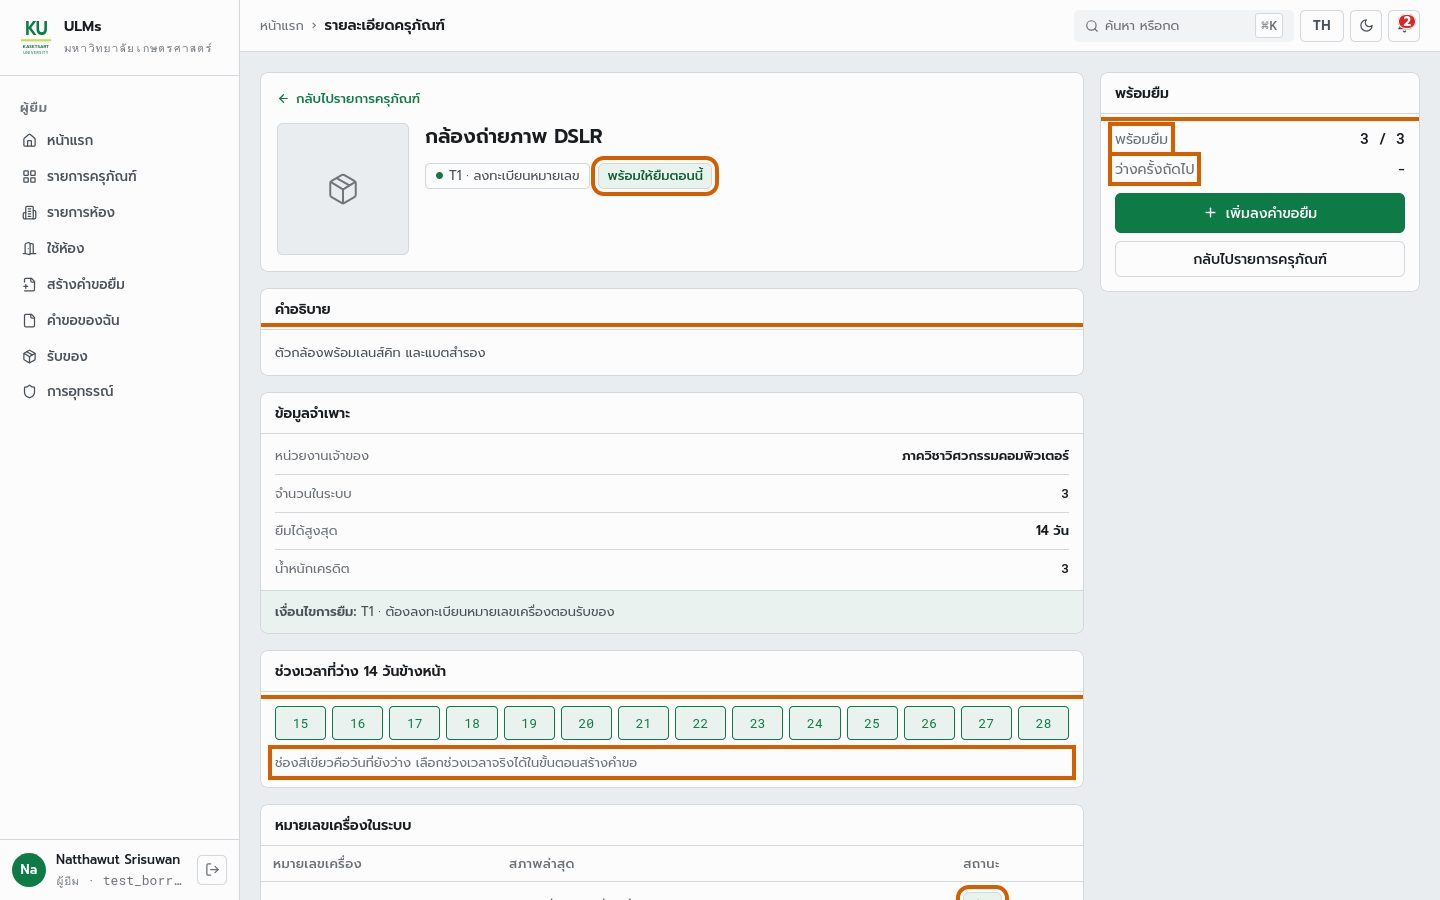
\includegraphics[width=\linewidth, trim={1100 610 20 72}, clip]{audit/b-detail-t1}\\[2pt]
{\sansall\scriptsize ผู้ยืม หน้ารายละเอียด: \textbf{3 / 3}}
\end{minipage}\hfill
\begin{minipage}[t]{0.6\textwidth}\centering
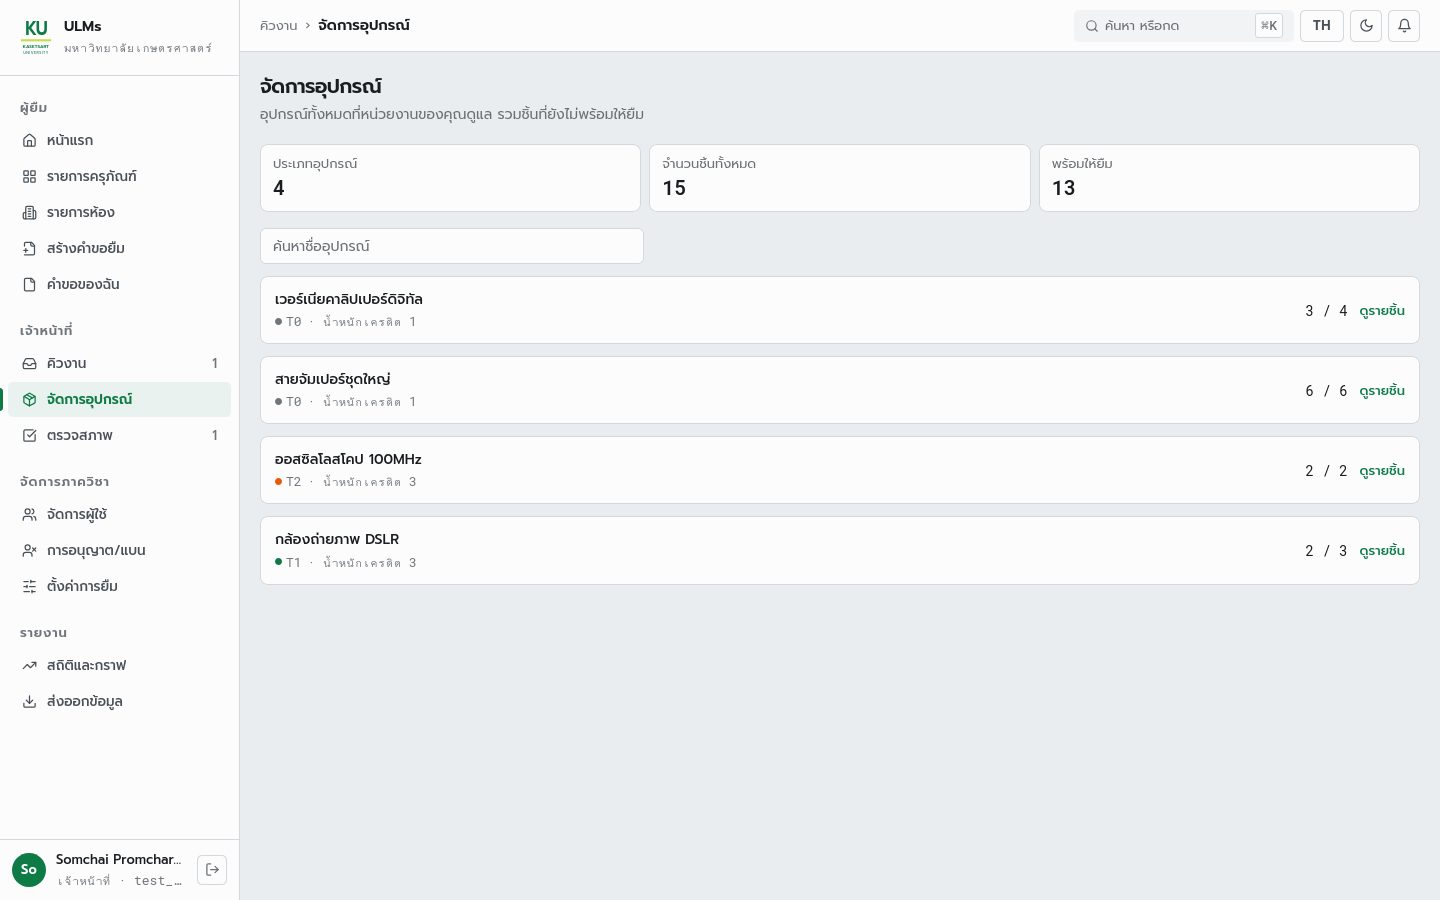
\includegraphics[width=\linewidth, trim={260 310 20 140}, clip]{audit/s-inventory}\\[2pt]
{\sansall\scriptsize เจ้าหน้าที่ หน้าจัดการอุปกรณ์: \textbf{2 / 3} (แถวล่างสุด)}
\end{minipage}
\end{figure}

\lab{ผล} ตัวนับฝั่งผู้ยืมลดตอนส่งมอบและเพิ่มกลับตอนรับคืน ฝั่งเจ้าหน้าที่ลดตอนจัดเตรียม ไม่มีฝั่งไหนลดตอนส่งคำขอหรืออนุมัติ
แต่ backend กันการจองตั้งแต่คำขอยังรออนุมัติ ถ้าย้ายไปนับตอนอนุมัติ ผู้ยืมจะเห็นว่าว่าง กดส่ง แล้วโดนปฏิเสธ

{\small
\begin{tabular}{L{4.3cm}cccccccc}
\toprule
\sansall\bfseries & ลงทะเบียน & ขอ & อนุมัติ & เตรียม & ส่งมอบ & รับคืน & ตรวจแล้ว \\
\midrule
ผู้ยืมเห็นว่าง & 3 & 3 & 3 & 3 & 2 & \textcolor{bad}{\textbf{3}} & 3 \\
เจ้าหน้าที่เห็นว่าง & 3 & 3 & 3 & 2 & 2 & 2 & 3 \\
\bottomrule
\end{tabular}
}

\issue{3}{เลือกวันยืมโดยไม่รู้ว่าวันไหนของเต็ม}{F01 F09}{BE FE}
\lab{สถานการณ์} นาย ก ขอกล้องวันที่ 16--18 ก.ย. แต่วันที่ 17 ทั้ง 3 ตัวถูกจองแล้ว หน้าจอขึ้นว่า ``ของว่างในช่วงที่ขอ'' และแถบ 14 วันเขียวทุกวัน

\begin{figure}[H]
\centering
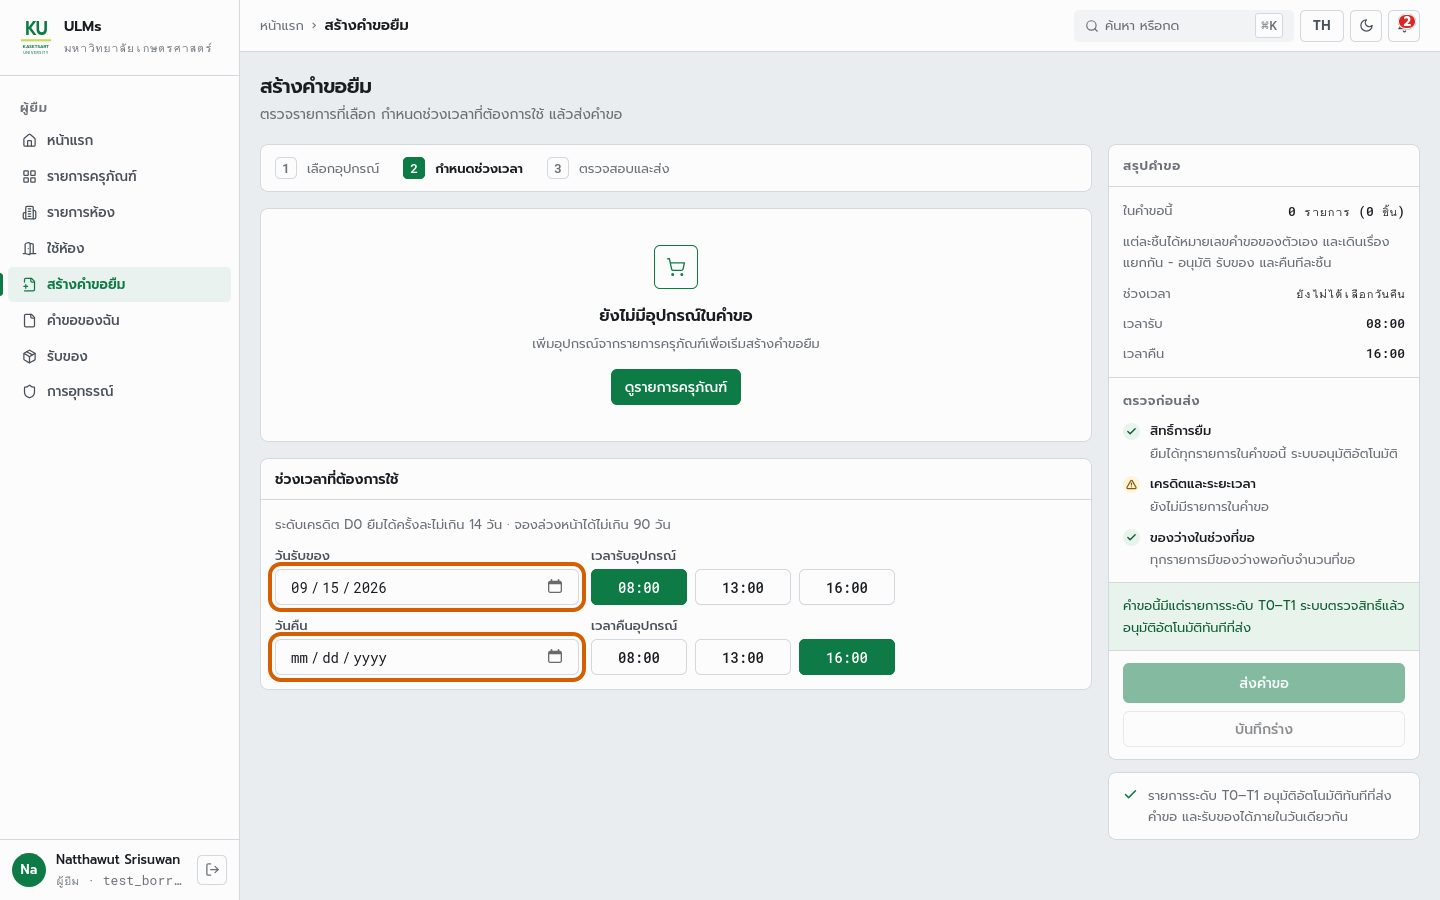
\includegraphics[width=0.82\textwidth, trim={240 200 0 50}, clip]{audit/b-request}\\[4pt]
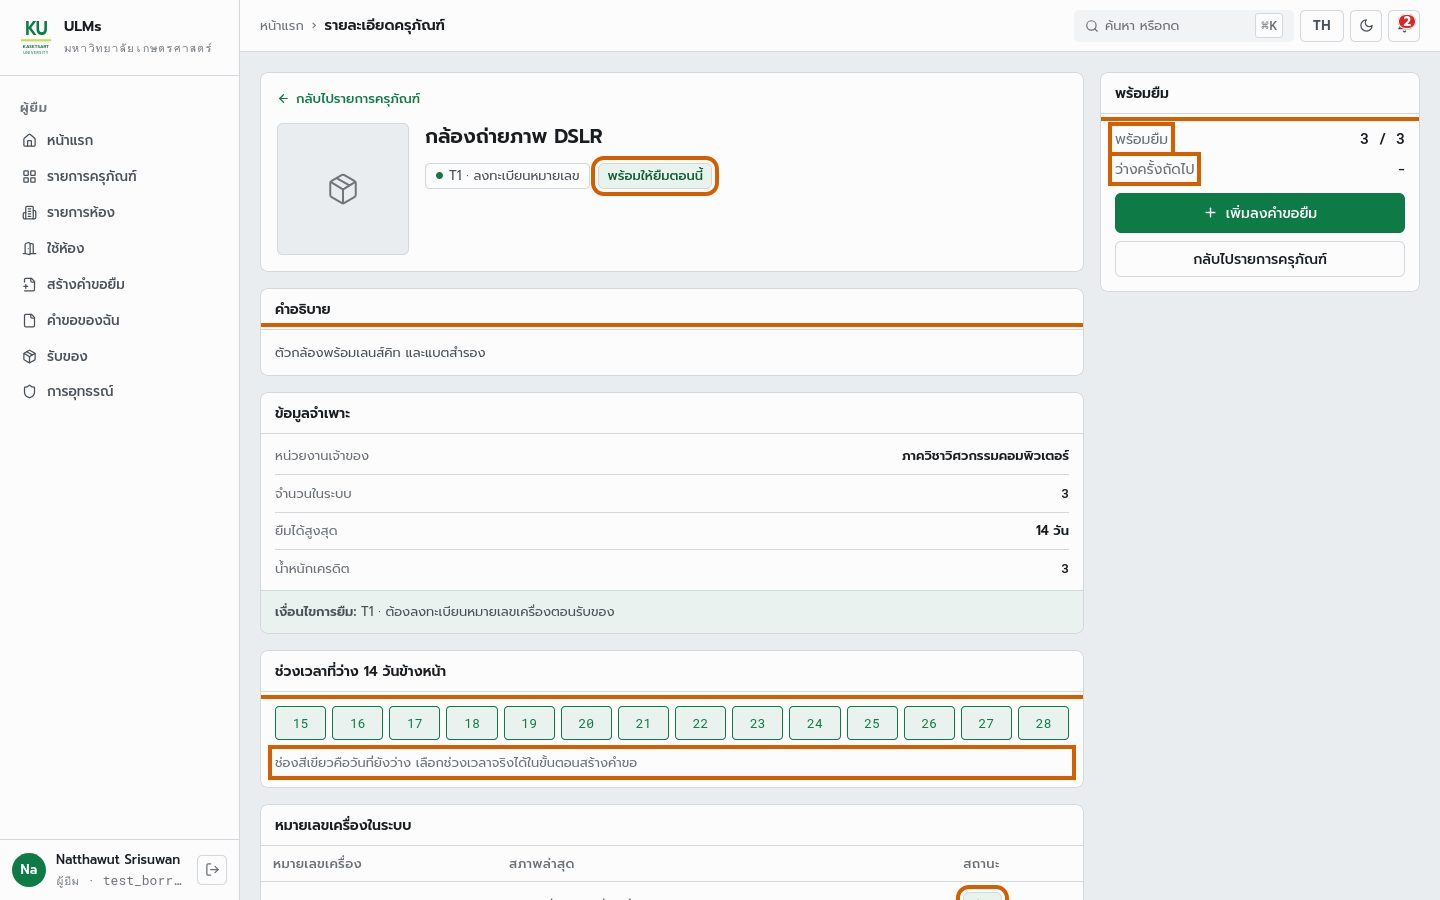
\includegraphics[width=0.82\textwidth, trim={260 110 355 650}, clip]{audit/b-detail-t1}
\end{figure}

\lab{ผล} หน้าคำขอมีแค่ช่องกรอกวันที่สองช่อง และเทียบจำนวนกับของว่าง ``ตอนนี้'' ไม่ใช่วันที่เลือก
แถบ 14 วันในหน้ารายละเอียดก็คิดจากตัวเลขตอนนี้ วันที่ถูกจองเต็มจึงยังเขียว

\issue{4}{ระบบไม่มีรูปตอนรับและตอนคืนเลย}{F05b F05c F13}{BE FE SA}
\lab{สถานการณ์} นิสิตคืนคาลิปเปอร์แล้วโดนประเมิน B2 นิสิตยืนยันว่ารอยมีตั้งแต่ตอนรับ เจ้าหน้าที่เปิดหน้าตรวจสภาพ เจอ ``ไม่มีรูป'' ทั้งสองฝั่ง

\begin{figure}[H]
\centering
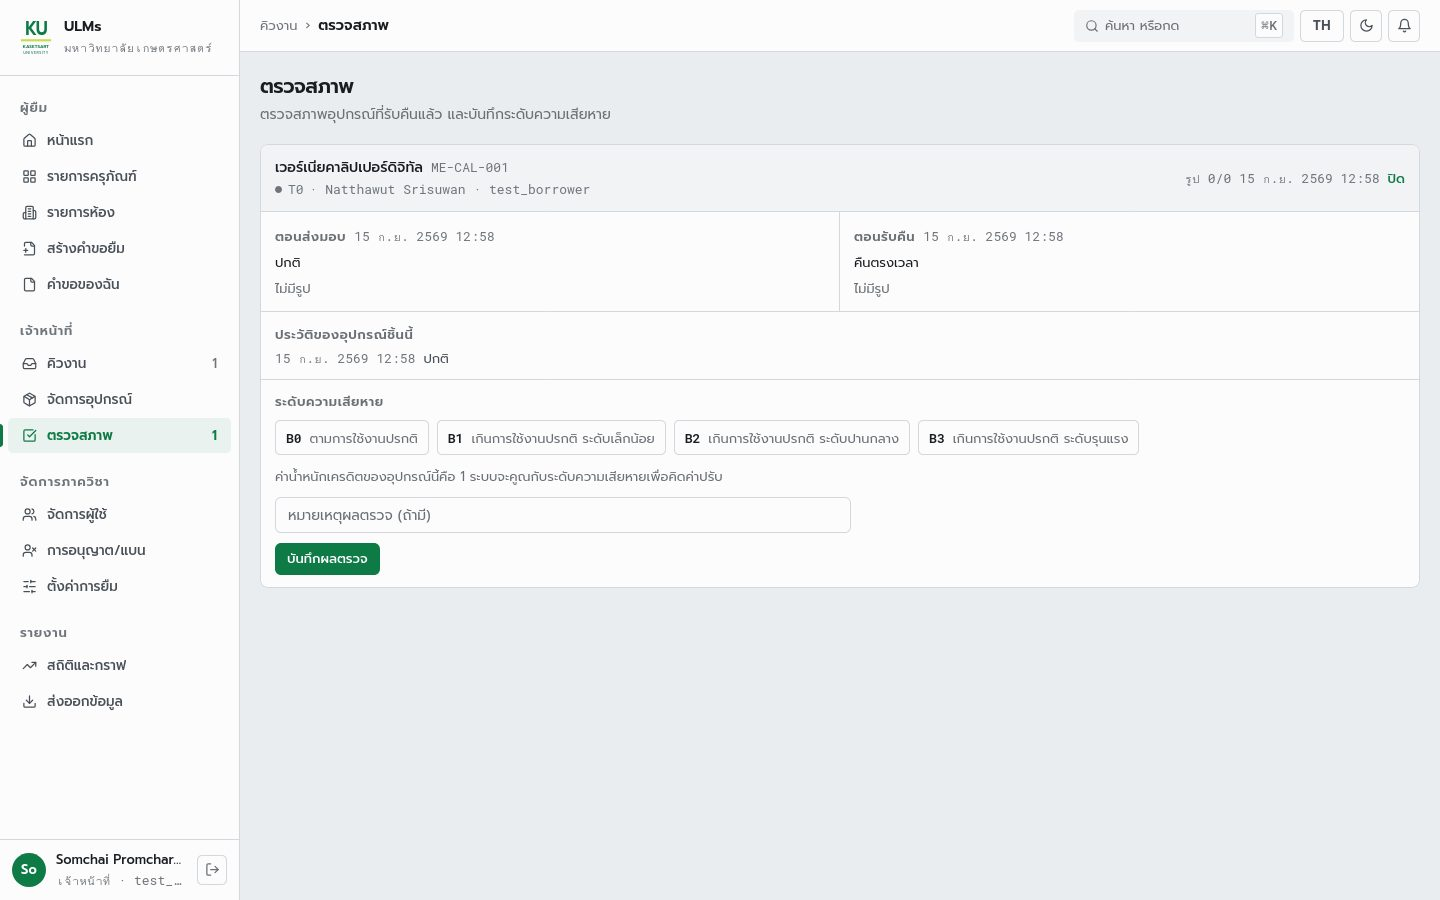
\includegraphics[width=0.88\textwidth, trim={240 300 0 60}, clip]{audit/s-inspection}
\end{figure}

\lab{ผล} หลังยืมครบวงจร 3 ครั้ง ตาราง \code{Images} มี 0 แถว
ผู้ยืมขออัปโหลดรูปได้ 403 เพราะ \code{image.requestUpload} ให้เฉพาะเจ้าหน้าที่ หน้ารับของบังคับถ่ายรูปแต่ไม่ส่งออกไป
\code{recordReturn} ของเจ้าหน้าที่ไม่มีช่องรับรูป ฟอร์มตรวจสภาพก็ไม่มีช่องแนบรูป
ถ้าทำตามข้อคิดเห็นให้ตัดรูปตอนรับทิ้ง กรณีแบบนี้จะไม่มีหลักฐานฝั่งผู้ยืมเหลืออยู่เลย

\issue{5}{อาจารย์อนุมัติเครื่อง A แต่เจ้าหน้าที่จ่ายเครื่อง B ได้}{F12}{BE}
\lab{สถานการณ์} ออสซิลโลสโคปมี A กับ B นิสิตขอ A อาจารย์อนุมัติ A เพราะ B เคยเสีย เจ้าหน้าที่จัดเตรียมโดยระบุ B ระบบรับ แล้วส่งมอบ B ออกไป

\lab{ผล} \code{swapUnit} ห้ามเปลี่ยนเครื่อง T2 แต่ \code{allocate} ทำเรื่องเดียวกันได้โดยไม่ตรวจ tier อาจารย์ไม่มีทางรู้ว่าเครื่องที่ออกไปไม่ใช่เครื่องที่อนุมัติ

\issue{6}{กฎห้อง 30 นาที × 6 ช่อง มีแค่บนหน้าจอ}{F03 F10}{BE FE SA}
\lab{สถานการณ์} เรียก API จองห้องตรง ๆ แบบ 14:00--17:30 (7 ช่อง) 13:10--13:40 (นอกกริด) 22:00--01:00 (ข้ามวัน) หรือจองล่วงหน้า 5 วัน

\lab{ผล} backend รับทั้งหมด ปฏิเสธเฉพาะช่วงที่ซ้อนกัน (ผิดกฎ 6 ใน 8 คำขอที่ทดสอบ แต่ถูกรับ)
ช่องว่าง/ไม่ว่างที่หน้าจองห้องแสดงเป็นข้อมูลตัวอย่าง ไม่ได้มาจากการจองจริง
SRS FR-REQ-08 ยังเขียนรายชั่วโมง 2 สล็อต และค่าคงที่ FE กับ \code{test:ac} ข้อ 2.6 ยังใช้กฎเก่า

\issue{7}{ห้องที่เจ้าหน้าที่เพิ่มเอง ไม่มีใครจองได้}{F23}{BE}
\lab{สถานการณ์} เจ้าหน้าที่เพิ่มห้อง 7603 ผ่าน \code{item.createRoom} นิสิตจองทันที ได้ \code{NOT\_ELIGIBLE / NO\_RULES\_CONFIGURED}

\lab{ผล} สิทธิ์จองต้องมีแถวใน \code{Eligibility} แต่ \code{item.setEligibility} รับแค่ประเภทอุปกรณ์ ห้องจึงไม่มีทางเปิดสิทธิ์
ห้องที่จองได้มีแค่ห้องที่มาจาก seed

\issue{8}{ลงทะเบียนของไม่มีหน้าจอ และเพิ่มจำนวนชิ้นพัง}{F06 F24}{FE BE}
\lab{สถานการณ์} ภาคได้ Arduino 30 ชิ้น เดือนถัดมาได้เพิ่มอีก 10 ชิ้น

\begin{figure}[H]
\centering
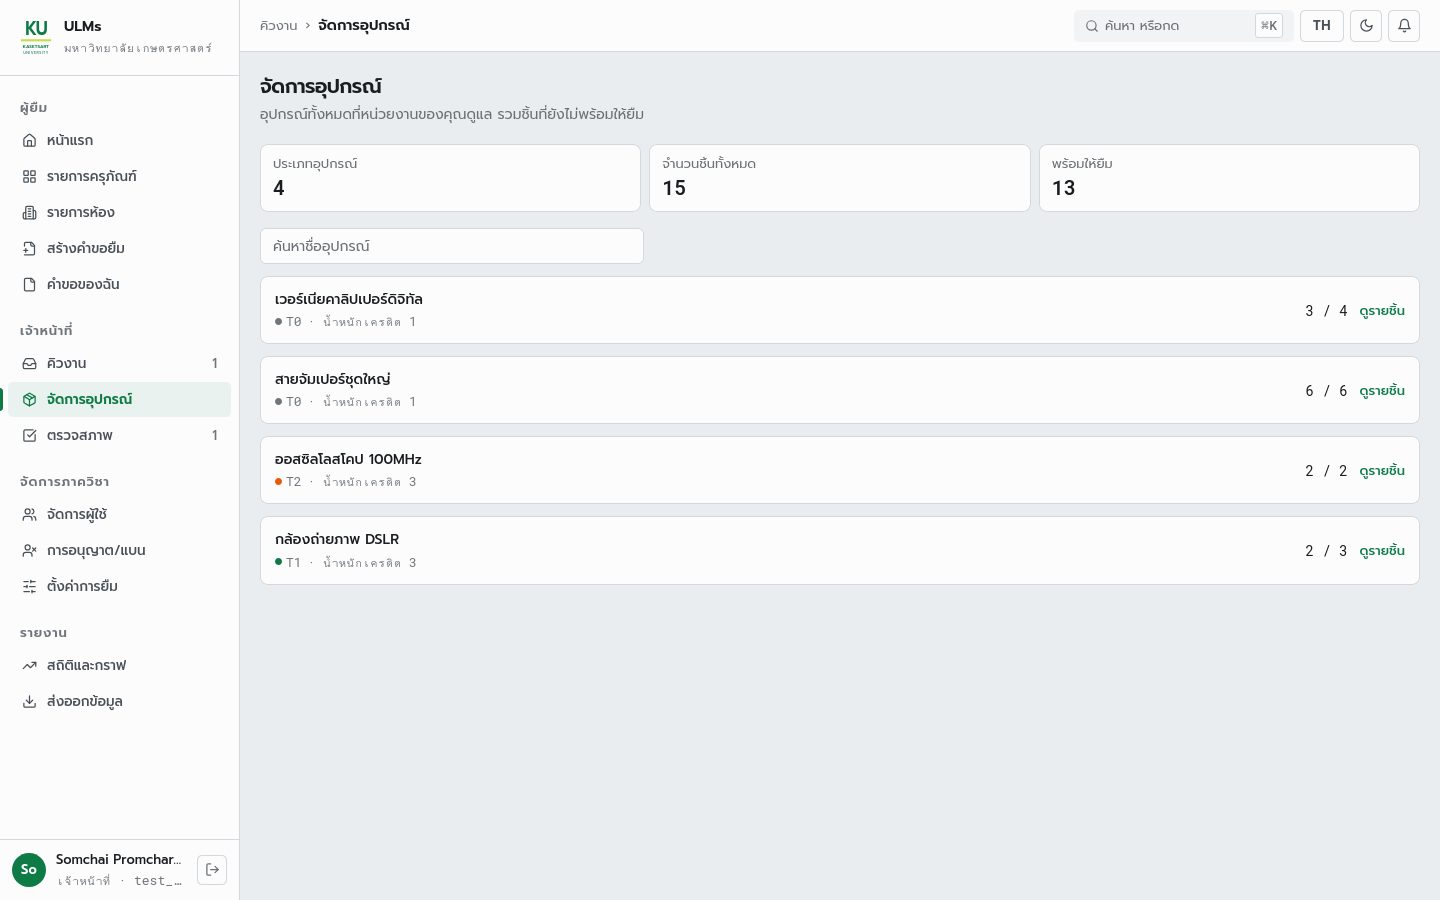
\includegraphics[width=0.78\textwidth, trim={240 300 0 60}, clip]{audit/s-inventory}
\end{figure}

\lab{ผล} หน้าจัดการอุปกรณ์ไม่มีปุ่มเพิ่มของหรือเพิ่มชิ้น ถ้าเรียก API เอง
\begin{itemize}
\item ของที่เพิ่งลงทะเบียนยังไม่มีใครยืมได้ จนกว่าจะเรียก \code{setEligibility} แยกอีกคำสั่ง
\item เพิ่มชิ้นให้ T0 เดิมได้ \code{SERIAL\_ALREADY\_IN\_USE} เพราะเลขที่ระบบสร้างเริ่มนับ 1 ใหม่ทุกครั้ง
\item เพิ่มชิ้นให้ T1 ได้ แต่ชิ้นใหม่ยืมไม่ได้เพราะไม่ได้สิทธิ์ตามชิ้นเดิม
\item T1 ยังถูกบังคับใส่ serial (\code{SERIAL\_REQUIRED\_FOR\_TIER}) ขัดข้อตัดสินของทีม
\end{itemize}

\issue{9}{ห้องไม่มีความจุ}{F02}{BE-lead SA}
\lab{สถานการณ์} อาจารย์ต้องการห้องสำหรับนิสิต 45 คน หน้าจองห้องแสดง ``40 ที่นั่ง'' แต่ตัวเลขนั้นมาจากข้อมูลตัวอย่าง

\begin{figure}[H]
\centering
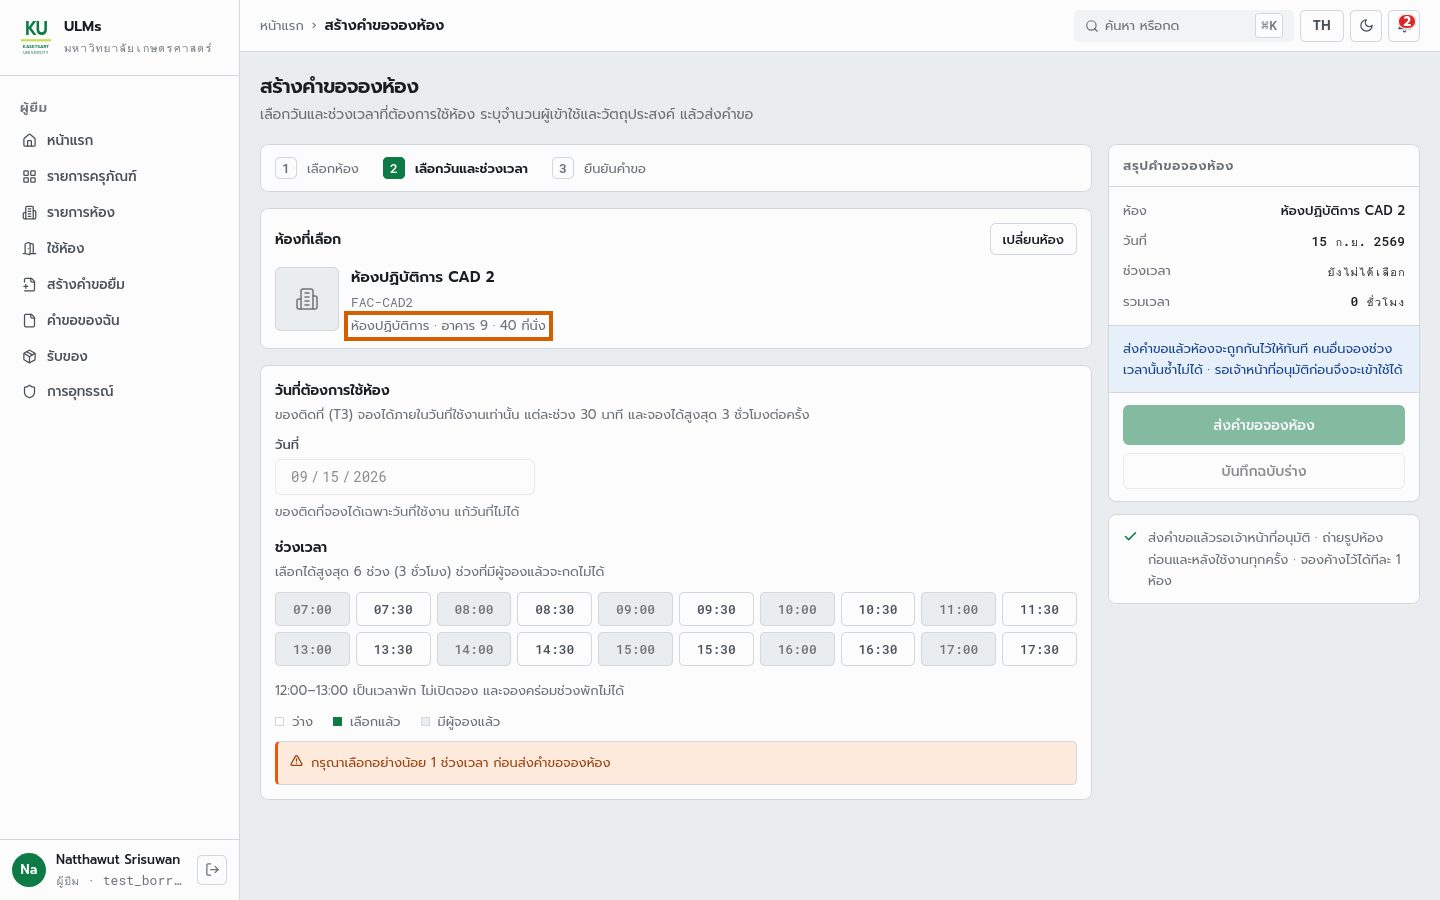
\includegraphics[width=0.8\textwidth, trim={240 520 0 60}, clip]{audit/b-room-booking}
\end{figure}

\lab{ผล} \code{RoomInfo} ไม่มีจำนวนที่นั่งหรือเวลาเปิด ห้องที่สร้างจริงจึงไม่มีความจุให้แสดง ขัด FR-EQP-04

\issue{10}{สัญญา API ฝั่ง FE ไม่ตรงของจริง}{F14}{FE}
\lab{สถานการณ์} FE จะทำหน้าลงทะเบียนตามข้อ 8 แต่ในสัญญามีแค่ \code{item.create} ซึ่ง backend ไม่มี และไม่มี \code{createType createUnit createRoom}

\lab{ผล} backend มี 86 procedure FE ประกาศ 74 ในนั้น 11 ตัวไม่มีจริง และมีของจริงอีก 23 ตัวที่ FE ไม่ได้ประกาศ
ซึ่งเป็นตัวที่ข้อ 3 4 6 8 ต้องใช้

% =============================================================================
\prio{pmid}{ความสำคัญกลาง}
% =============================================================================

\issue{11}{ระบบมีการแบนการยืม ซึ่งไม่มีในแผน}{F17}{BE FE SA}
\lab{สถานการณ์} เจ้าหน้าที่เปิดเมนู ``การอนุญาต/แบน'' แบนนิสิตคนหนึ่ง 7 วัน นิสิตกดส่งคำขอยืม ระบบปฏิเสธด้วย \code{BORROWING\_SUSPENDED}

\lab{ผล} ตามแผน บทลงโทษมีผลผ่านแถบเครดิต D0--D3 เท่านั้น คือจำกัดจำนวนวันยืมและเปลี่ยนเส้นทางการอนุมัติ (FR-CRD-08)
ส่วน FR-ADM-03 คือผู้ดูแลระบบปิดบัญชีทั้งบัญชี ไม่ใช่การห้ามยืม
แต่โค้ดมี \code{admin.setUserBan} ที่เจ้าหน้าที่ใช้ได้ พร้อมหน้าจอและ e2e test ของมัน (TP-ADM-E2E-05/06)
และ SDS v1.1 ก็เขียนการระงับการยืมไว้ตามโค้ด
ผลข้างเคียง ถ้านิสิตมีโทษจากของเสียอยู่ด้วย การยกเลิกแบนจะปิดโทษความเสียหายไปพร้อมกัน (\code{admin.service.ts:450})

\lab{อีกสองจุดในหมวดเครดิต} เครดิตถูกลบตรงแทนการคำนวณจากโทษที่ยังมีผล จึงไม่คืนเมื่อโทษถูกปิด (ขัด FR-CRD-06)
และเมื่ออาจารย์ปฏิเสธคำขอ เหตุผลของผู้ยืมถูกเขียนทับด้วยเหตุผลที่ปฏิเสธ (\code{approval.service.ts:253})
การปฏิเสธคำขอของคนที่ถูกแบนและสองจุดนี้ยืนยันจากโค้ด ยังไม่ได้รันสถานการณ์จริง

\issue{12}{อุทธรณ์ยังไม่มีระบบ อาจารย์แทบไม่มีงาน}{F18 F19}{BE FE}
\lab{สถานการณ์} นิสิตไม่เห็นด้วยกับผล B2 กดยื่นอุทธรณ์ อาจารย์เปิดหน้าอุทธรณ์ เจอข้อมูลตัวอย่างที่มีแถบแจ้งว่ายังไม่มีระบบหลังบ้าน

\begin{figure}[H]
\centering
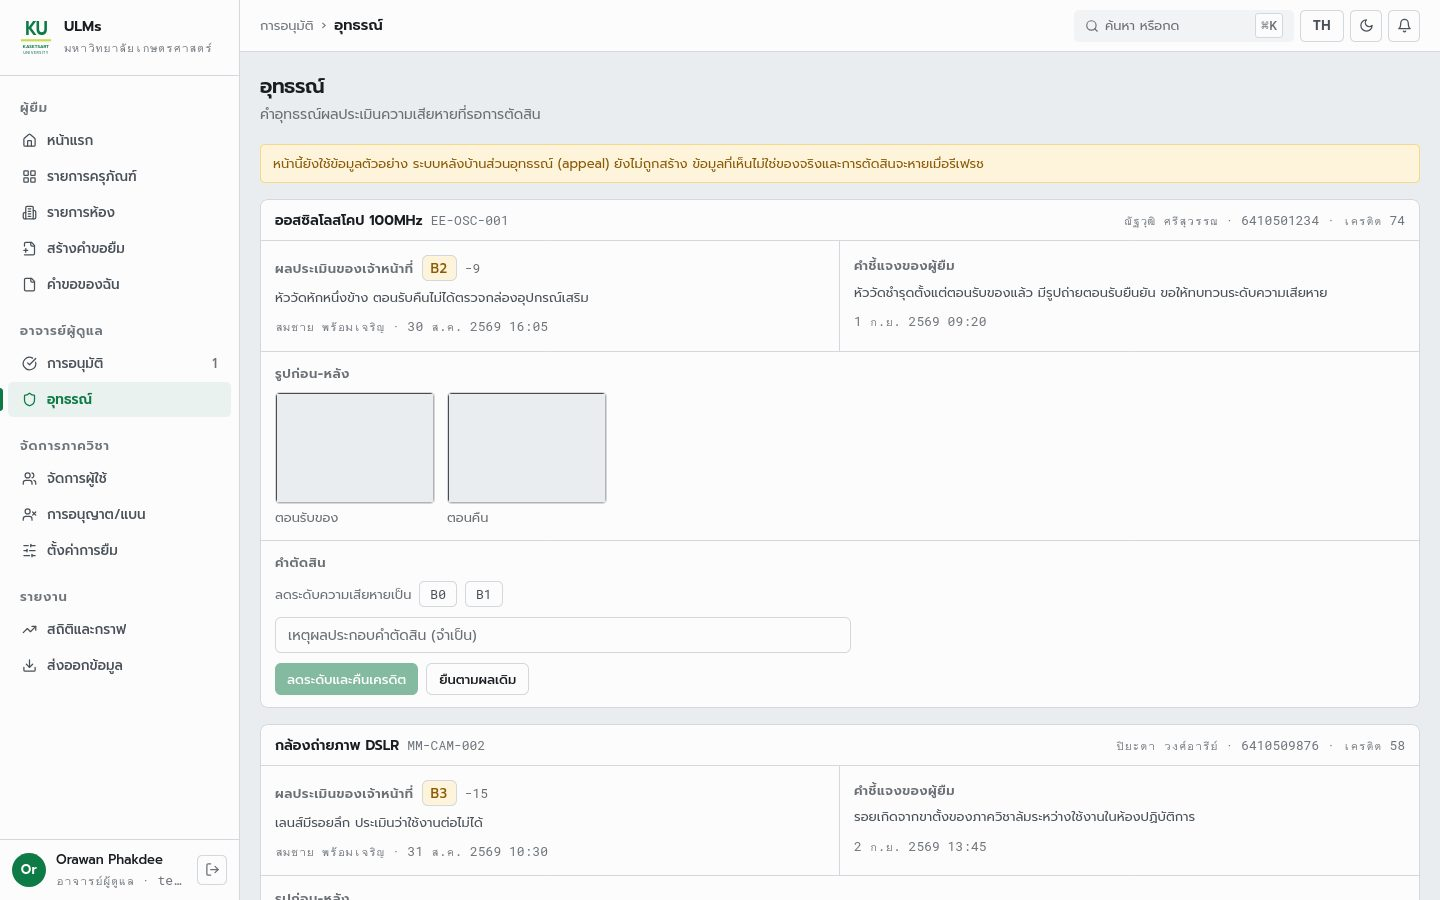
\includegraphics[width=0.85\textwidth, trim={240 560 0 60}, clip]{audit/v-appeals-mock}
\end{figure}

\lab{ผล} backend ไม่มี router อุทธรณ์ FR-APL ทั้ง 6 ข้อยังไม่ทำงาน
อาจารย์เหลืองานจริงแค่อนุมัติ T2 ขัดเกณฑ์ของอาจารย์ที่ให้ทุกบทบาทมีงาน

\issue{13}{บันทึกการใช้งานไม่มีการยืม อนุมัติ ตรวจสภาพ}{F26}{BE}
\lab{สถานการณ์} มีข้อพิพาทว่าใครอนุมัติคำขอ หรือใครให้ระดับความเสียหาย ผู้ดูแลระบบเปิดบันทึกการใช้งาน

\begin{figure}[H]
\centering
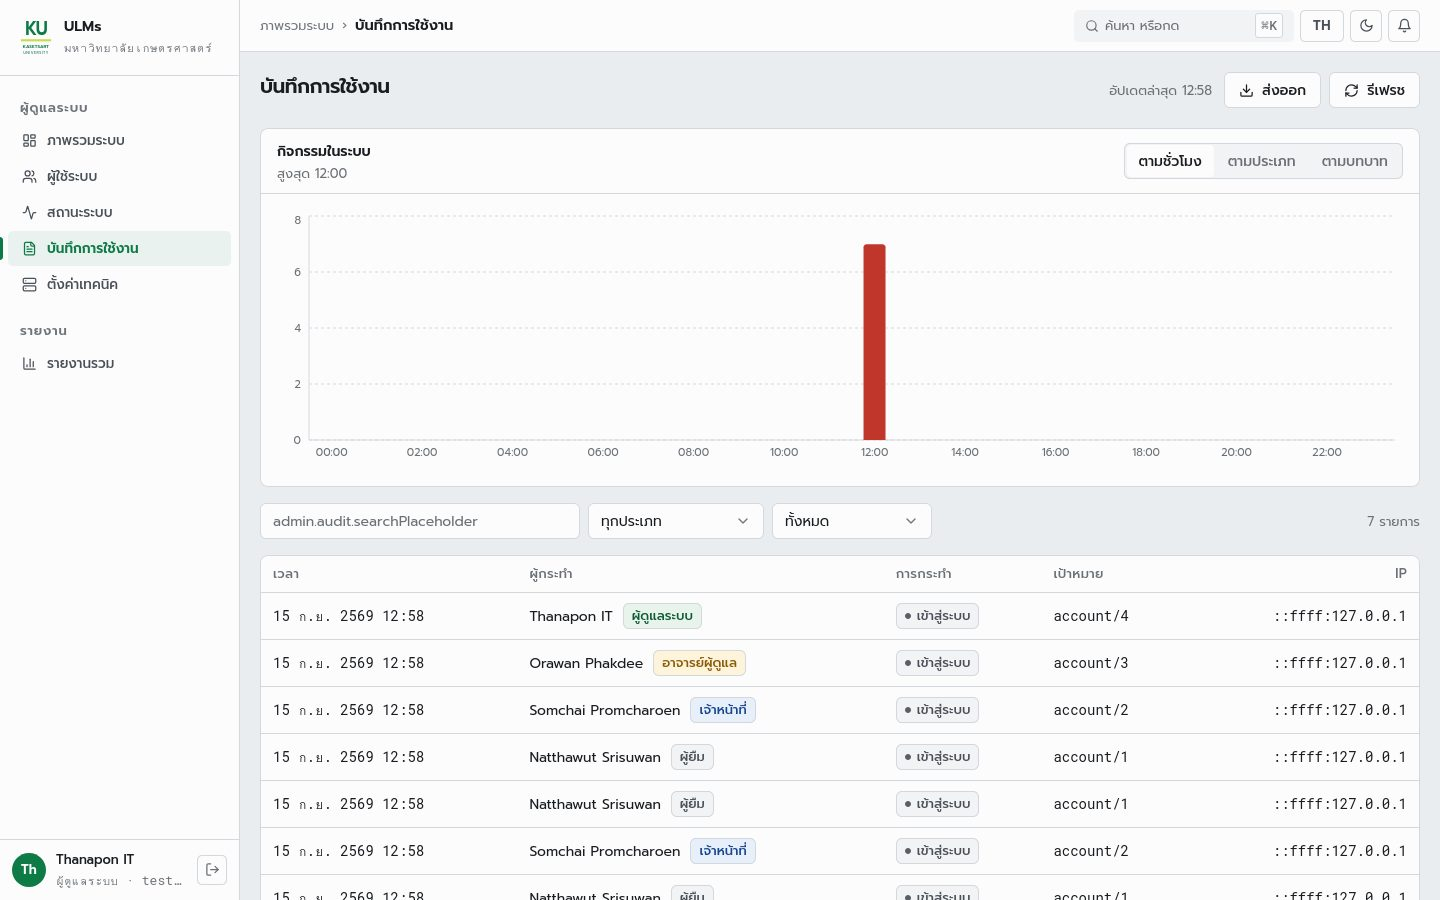
\includegraphics[width=0.85\textwidth, trim={240 240 0 490}, clip]{audit/a-audit}
\end{figure}

\lab{ผล} หลังมีคำขอ 15 ใบ บันทึกมีแค่ login 30 แถว update 6 แถว role 2 แถว
โมดูล loan approval inspection item ไม่บันทึกเลย ขัด FR-ADM-05

\issue{14}{test ผ่านหมด แต่ไม่มีชุดไหนแตะวงจรยืม}{F21}{ทีม test}
\lab{สถานการณ์} ปัญหาข้อ 2 5 6 7 8 11 ทั้งหมดอยู่ในโค้ดตอนที่ test ผ่านครบ

\lab{ผล} backend 266/266 frontend 33/33 และ 49/49 e2e ผ่าน 10 แต่ไม่มี test ของ loan approval inspection

% =============================================================================
\prio{plow}{ความสำคัญต่ำ}
% =============================================================================

\issue{15}{ป้าย ``ถูกระงับ'' ไม่ตรงความจริง}{F25}{BE FE}
\lab{สถานการณ์} นิสิตมีโทษหักเครดิตจากของเสีย หน้าผู้ใช้ของเจ้าหน้าที่ขึ้น ``ถูกระงับ'' แต่นิสิตยังส่งคำขอยืมได้ปกติ

\lab{ผล} แผนไม่มีสถานะระงับ นิสิตที่มีโทษเครดิตแค่ถูกลดวันยืมหรือเปลี่ยนผู้อนุมัติ แต่ป้ายนับโทษทุกชนิดเป็น ``ถูกระงับ''

\issue{16}{สถานะของผู้ยืมสองแบบไม่มีวันขึ้น}{F08}{BE FE}
\lab{สถานการณ์} นิสิตคืนของแล้วเปิดดูคำขอของฉัน อยากรู้ว่าของกำลังถูกตรวจ

\lab{ผล} ``กำลังจัดเตรียม'' ไม่เกิดเพราะไม่มีโค้ดใดเขียนสถานะนั้น
``รอตรวจสภาพ'' มีแค่ฝั่ง FE backend ส่ง \code{returned} มาแทน

\issue{17}{สร้างประเภทอุปกรณ์ไม่ตรวจหน่วยงาน}{F13}{BE}
\lab{สถานการณ์} เจ้าหน้าที่ภาคไฟฟ้าสร้างประเภทอุปกรณ์ใหม่

\lab{ผล} \code{createType} ไม่ตรวจว่าผู้เรียกอยู่หน่วยงานไหน ต่างจากการสร้างห้องและการแก้ประเภทที่ตรวจ ขัดหลัก FR-AUTH-05

\issue{18}{ค่าเครดิตบนหน้าจอคิดด้วยตัวเลขคงที่}{F15}{FE}
\lab{สถานการณ์} กล้อง DSLR ในระบบมีน้ำหนักเครดิต 3 แต่หน้าผู้ยืมคำนวณค่าหักด้วย T1 = 5

\lab{ผล} ค่าหักที่ผู้ยืมเห็นไม่ตรงกับที่ระบบหักจริง และของที่ไม่รู้ tier ถูกแสดงเป็น T2

\issue{19}{ข้อความ เมนู และหน้าที่ยังว่าง}{F16 F18 F22}{FE}
\lab{สถานการณ์} ผู้ดูแลระบบเปิดหน้าบันทึกการใช้งาน ช่องค้นหาขึ้นว่า \code{admin.audit.searchPlaceholder} (ดูภาพข้อ 13)
เจ้าหน้าที่กับอาจารย์ยืมของได้แต่เมนูไม่มี ``รับของ'' ``อุทธรณ์'' ``ใช้ห้อง'' และหน้าส่งมอบกับหน้าส่งออกข้อมูลเปิดเข้าไปแล้วว่าง

\begin{figure}[H]
\centering
\begin{minipage}[t]{0.48\textwidth}\centering
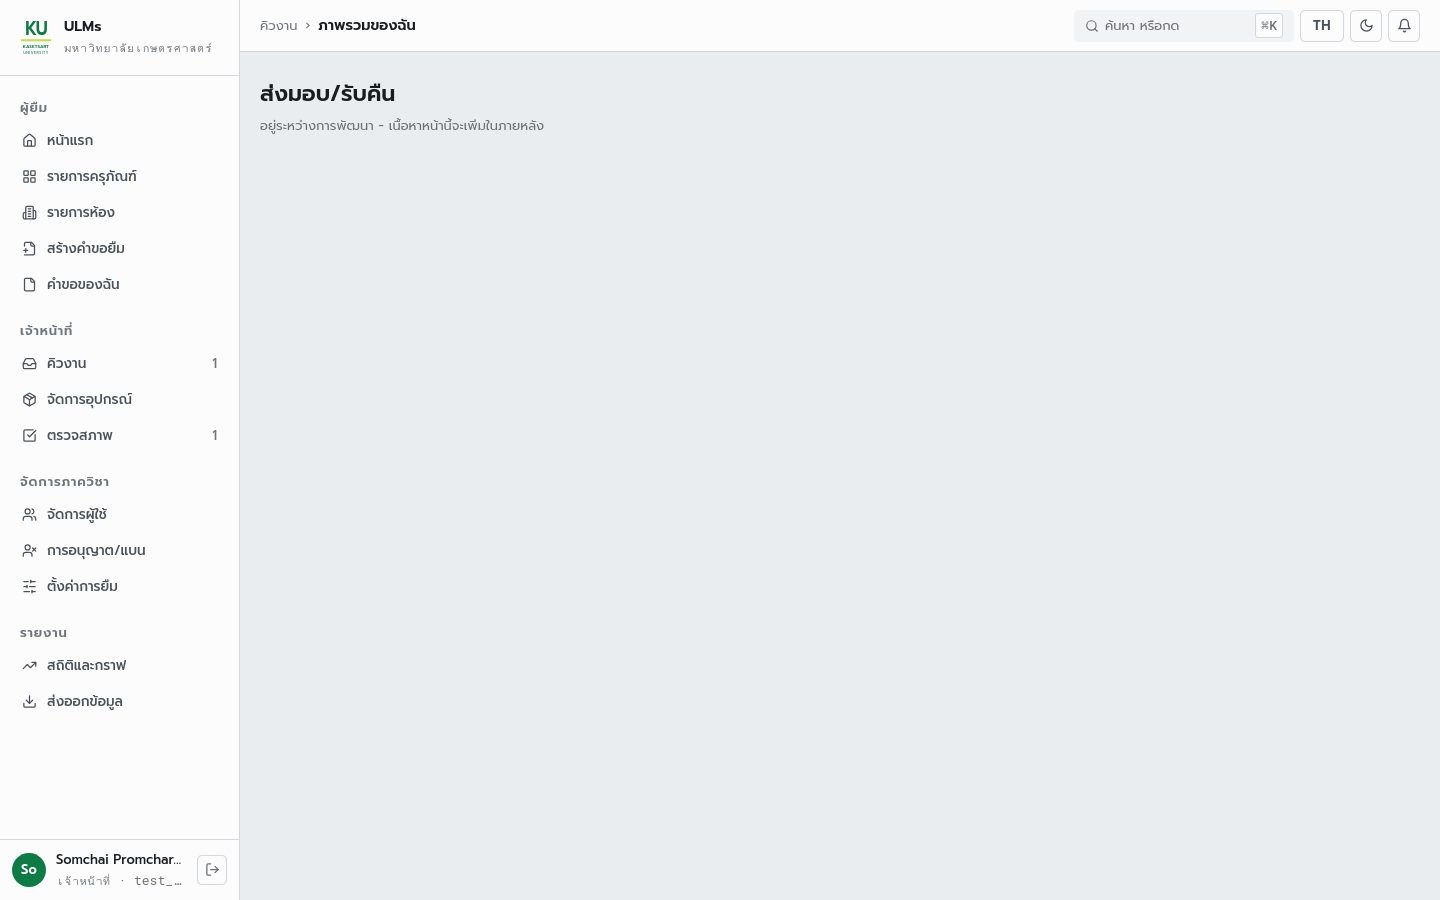
\includegraphics[width=\linewidth, trim={240 450 0 0}, clip]{audit/s-handover-placeholder}\\[2pt]
{\sansall\scriptsize \code{/staff/handover}}
\end{minipage}\hfill
\begin{minipage}[t]{0.48\textwidth}\centering
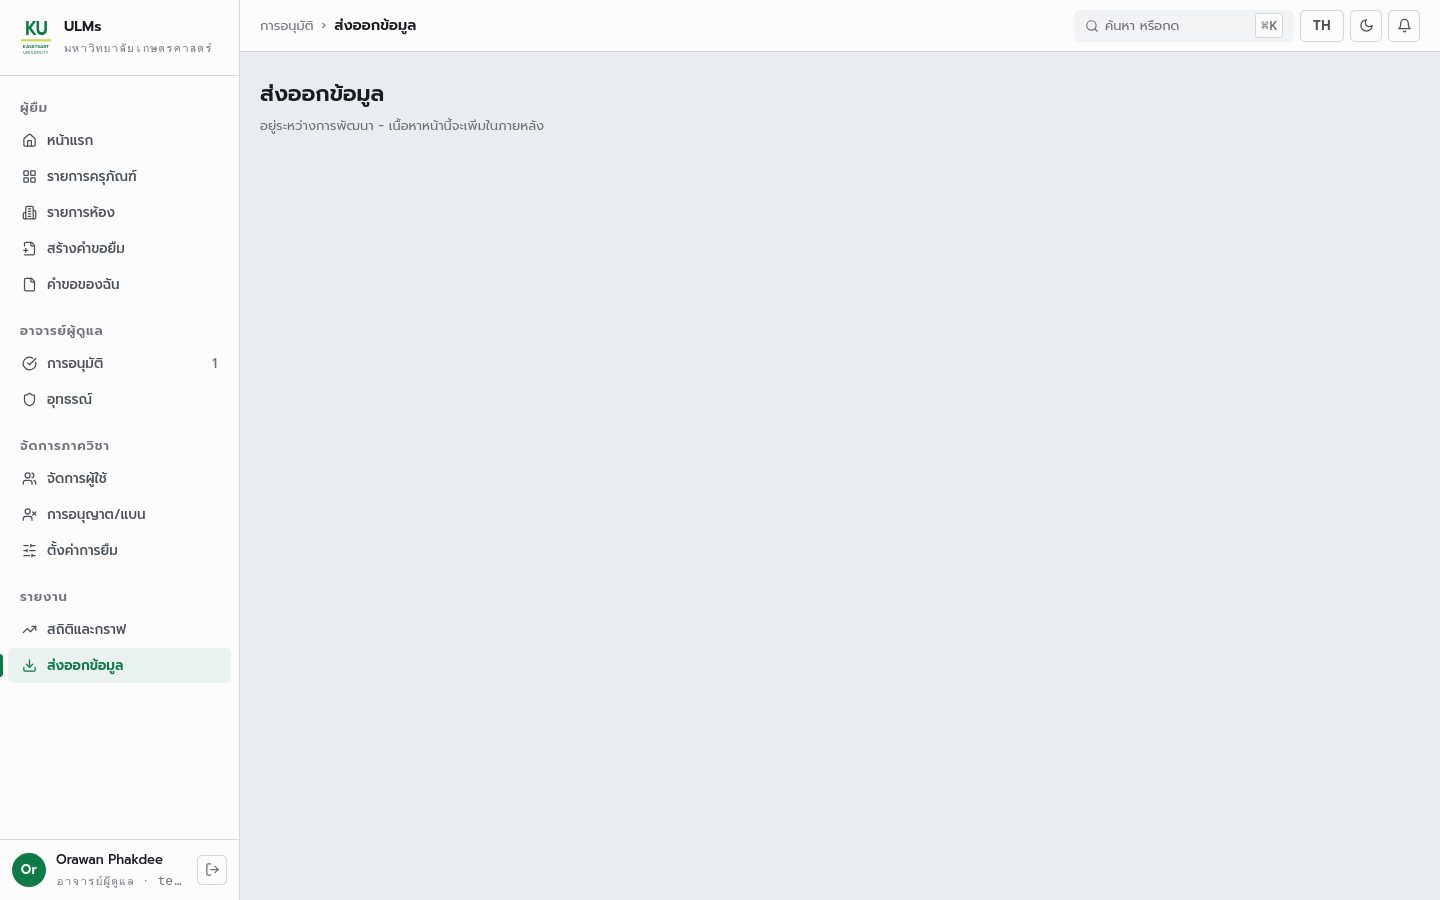
\includegraphics[width=\linewidth, trim={240 450 0 0}, clip]{audit/v-export-placeholder}\\[2pt]
{\sansall\scriptsize \code{/reports/export}}
\end{minipage}
\end{figure}

% =============================================================================
\section*{เรื่องที่ SA ต้องตัดสิน}
\markboth{เรื่องที่ SA ต้องตัดสิน}{}
% =============================================================================

{\small
\begin{tabular}{L{0.6cm}L{13.7cm}}
\toprule
1 & ของถูกกันเมื่อไร SDS ว่าตอนส่งคำขอ FR-APV-05 ว่าตอนอนุมัติ ข้อเสนอโครงการว่าตอนจัดเตรียม \\
2 & ห้อง T3 ใครอนุมัติ SRS ไม่มีข้อ ข้อเสนอโครงการว่าอัตโนมัติ โค้ดส่งให้เจ้าหน้าที่ \\
3 & เครดิตต้องคำนวณจากโทษที่ยังมีผลตาม FR-CRD-06 หรือเก็บเป็นตัวเลขอย่างที่โค้ดทำ \\
4 & การต่ออายุ D2--D3 และ T3 ต่างจาก SRS (ค้างจากรอบก่อน) \\
5 & FR ที่ขัดกับข้อตัดสินของทีม: FR-REQ-08 FR-EQP-03 FR-EQP-04 FR-EQP-06 FR-PKP-01 FR-PKP-04 FR-RTN-01 และยังไม่มี FR ปฏิทินของอุปกรณ์ \\
6 & SDS v1.1 เขียนการระงับการยืมไว้ตามโค้ด (กรณีใช้งานส่งคำขอ และรายการ \code{setUserBan}) ขัด SRS ที่ไม่มีการแบน \\
\bottomrule
\end{tabular}
}

\end{document}
